\chapter{Dataset}
\label{ch:dataset}

How do we efficiently create, organise and use labelled datasets to permit useful machine learning? What is a label, and how can we constrain them? In this chapter, we present a offers the metamodel that offers the conceptual vocabulary and an organising principle to improve efficiency of labelling.

\section{A Data-Capturing Metamodel}
\label{sec:dataset:architecture}

Why should we care about the architecture of our dataset capturing, so long as the \gls{ai} is well-trained? This question fundamentally leads to the \textit{provenance} or \textit{lineage} of our data: not all training data is initially perfect. At times, we will need to modify our training data, or in the cases of some \gls{ai} systems, training data is re-fed back into the system from the \gls{ai} itself. 

Hence, it is imperative to understand how the transition and flow of data occurs \citep{Cui:2003im,Ikeda:2009ca,Buneman:2000bn} in these \gls{ai} systems. Where does it comes from? How is it derived and updated, and how might this affect our trained \gls{ai} models over time? Without a thorough understanding of data provenance, tracing potential defects within training models becomes difficult. It may be a difference in the data training format, or a mismatch of values on the same training data. Systematic record-keeping is critical to overcome this challenge.

We propose a grammar to capture the vocabulary of our metamodel and the approach of developing a data-capturing architecture. As such a grammar is textual, it can be version controlled: therefore data provenance is recorded, which allows us to source how the mutations in training data can occur and and what effect this has our \gls{ai} systems. From an exploratory analysis of developing a concrete implementation of this system (\cref{sec:dataset:architecture:methodology}), we propose a conceptual metamodel that can be used to annotate and formally describe image data for training purposes (e.g., frames of a video, images of natural scenes). This metamodel is inspired by the works of \citet{Wickham:2010hy, Wickham:2007tu} and \citet{Moody:2009vo}.

\subsection{Methodology}
\label{sec:dataset:architecture:methodology}

To understand the methodology on how we captured our dataset, we must first introduce the three key notions behind \gls{mde}: technical spaces, models and systems. A system is a concrete ``group or set of related or associated elements perceived or thought of as a unity or complex whole'' \citep{oed:system}. Technical spaces were introduced \citet{Bezivin:2002} as a model management framework based on algebraic structures (e.g., trees, (hyper)graphs, categories). Technical spaces are usually based on a three-tier conjecture: metametamodels, metamodels and models. Whereas a model is an abstract representation a concrete system of specific purpose, a \textit{meta}model, in contrast, describes the way to describe those models. A \textit{metameta}model can be used to describe the representation structure of our metamodels and defines a type system that supports all underlying layers \citep{Bezivin:2006gw}. \cref{fig:dataset:bezivin2006_metamodel} captures these concepts in further detail.

\begin{figure}[h]
  \centering
  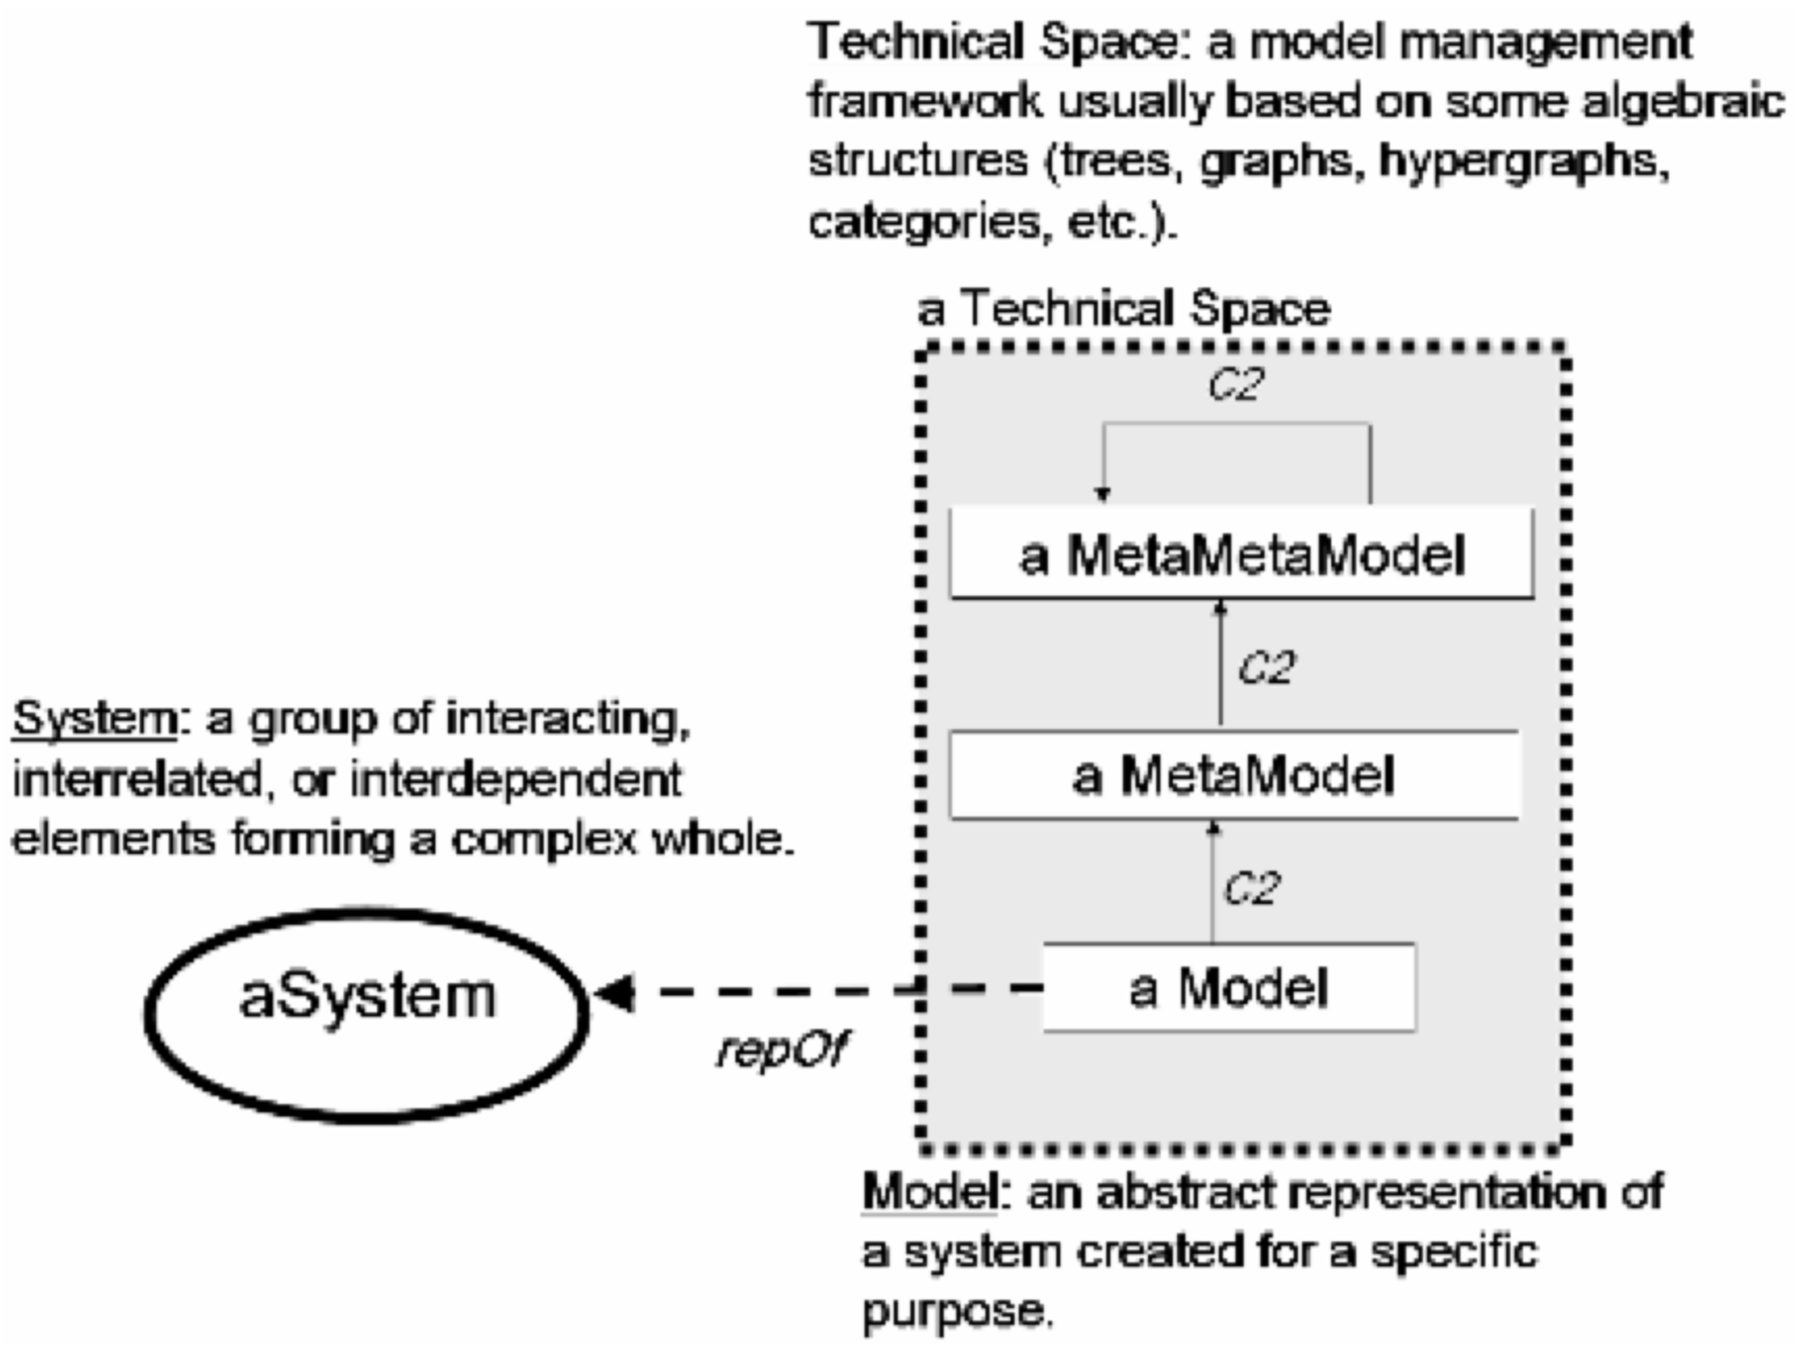
\includegraphics[width=0.6\textwidth]{images/dataset/bezivin2006_metamodel}
  \caption[An overview of systems, models and technical spaces]{Systems, models and technical spaces. (From \citep{Bezivin:2006gw}.)}
  \label{fig:dataset:bezivin2006_metamodel}
\end{figure}

We captured these concepts in a prototypical exploration process, first by developing a prototype system iteratively with a data tagging team who manually curated the data. Once this prototype was stable, we developed a model (\cref{sec:dataset:architecture:what_to_capture}) around the prototype. We generalised the system we had developed, expanding from a model we had designed that was marathon-specific, into a more generalisable metamodel (\cref{sec:dataset:architecture:metamodel}). We represent our process as as a \gls{uml} activity sequence diagram, shown in \cref{fig:dataset:methodology}.

The initial phase in our dataset development was to create a prototype system with the specific purpose of tagging our marathon runner context (using the dataset provided by the industry client). We name this partial implementation \textit{Argus}\footnoteurl{http://www.deakin.edu.au/~ca/argus}{5 July 2017}\footnote{Whose name is inspired by the \textit{all-seeing} giant of the same name from Greek mythology: ``With his multiple sets of eyes, Argus could see nearly everything in his vicinity''. See \url{http://www.loggia.com/myth/argus.html}.}. Refer to \cref{sec:dataset:argus} for more about this implementation. 

To develop this initial model (and thus to then what our metamodel would be), we began by discussing what requirements were needed---that is, the key features that we thought were necessary for extracting from our image. Five features were decided: (1) the crowdedness of the photo, (2) the visible bib sheets within the photo, (3) the faces corresponding to those bib sheets, (4) the prominence of runners of the photo and (5) the colours of runners' clothing in the photo.

Once an initial prototype was developed, we conducted informal usability tests with members from \gls{dstil}, which captured minor flaws in the workflow (namely required conditions that were missing in annotations) as well as general usability enhancements. Once the internal testing had concluded, we developed instructional video guides on how to use Argus, and then deployed the tool to a data tagging team that made the data available to us.

After deployment, we ran four iterations of tagging with our external data tagging team. We use the term \textit{iteration} to refer to the process of deploying Argus to the data tagging team, capturing a set of photos from various races, and sending the data back for quality assurance. These iterations consisted of photos from different marathon races in our dataset. (To ensure variance in tagging, there were some races at night and some races with alphanumeric components in the \gls{rbn}.) After each iteration we assessed the tagging for quality. Feedback identified further restrictions that needed to be placed on Argus as poor approximations or incorrect tagging would cause our \gls{ai} to learn poorly. 

The following issues were identified:

\begin{itemize}
  \item face region was too far away from the bib region,
  \item face region was overlapping the bib region,
  \item \glspl{rbn} had spaces,
  \item misidentified \glspl{rbn} where the alphabetic `I' was tagged as the numeric `1'.
\end{itemize}

\noindent
Furthermore, we added geometric restrictions and conditions into the tool to prevent these errors from occurring at all (i.e., ensuring faces could only be marked above and horizontally near bibs). Some of these issues are highlighted in \cref{fig:dataset:issues_with_tagging}.

\begin{figure}[p]
  \centering
  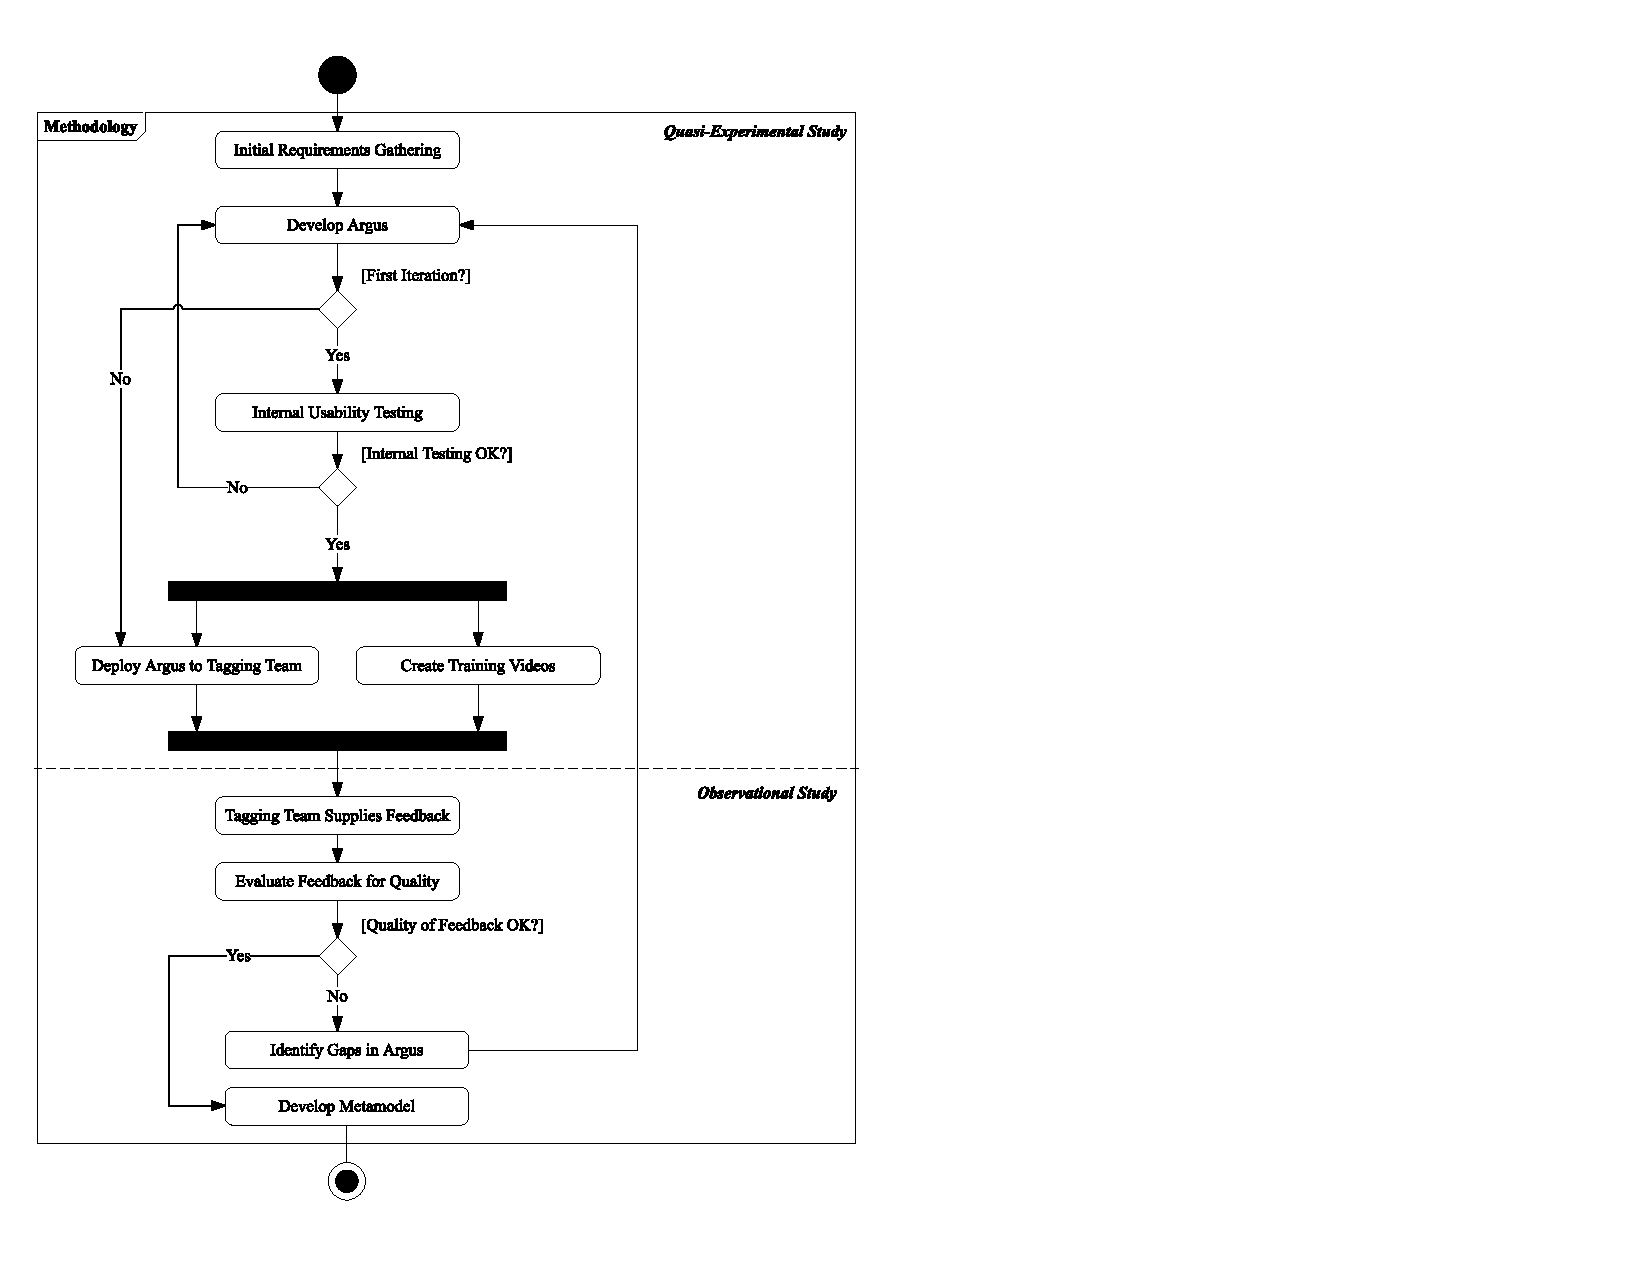
\includegraphics[width=0.7\textwidth]{images/dataset/methodology}
  \caption[Implementation methodology]{An overview of the methodology used to discover our metamodel.}
  \label{fig:dataset:methodology}
\end{figure}

\begin{figure}[p]
  \centering
  
  \begin{subfigure}[b]{0.8\textwidth}
    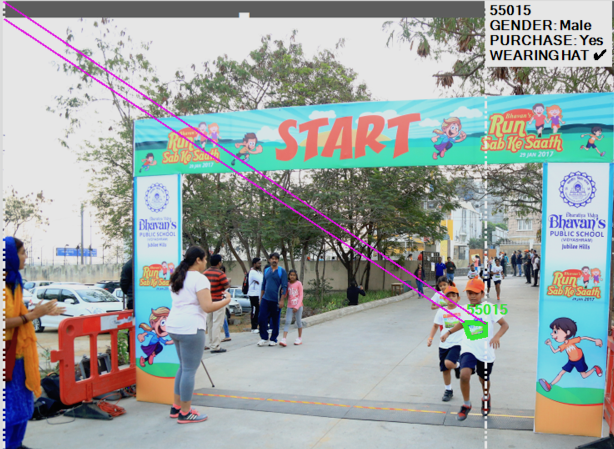
\includegraphics[width=\textwidth]{images/dataset/BadTagging_TooFar}
  \end{subfigure}\\
  \vspace{1cm}
  \hspace{\fill}
  \begin{subfigure}[b]{0.3\textwidth}
    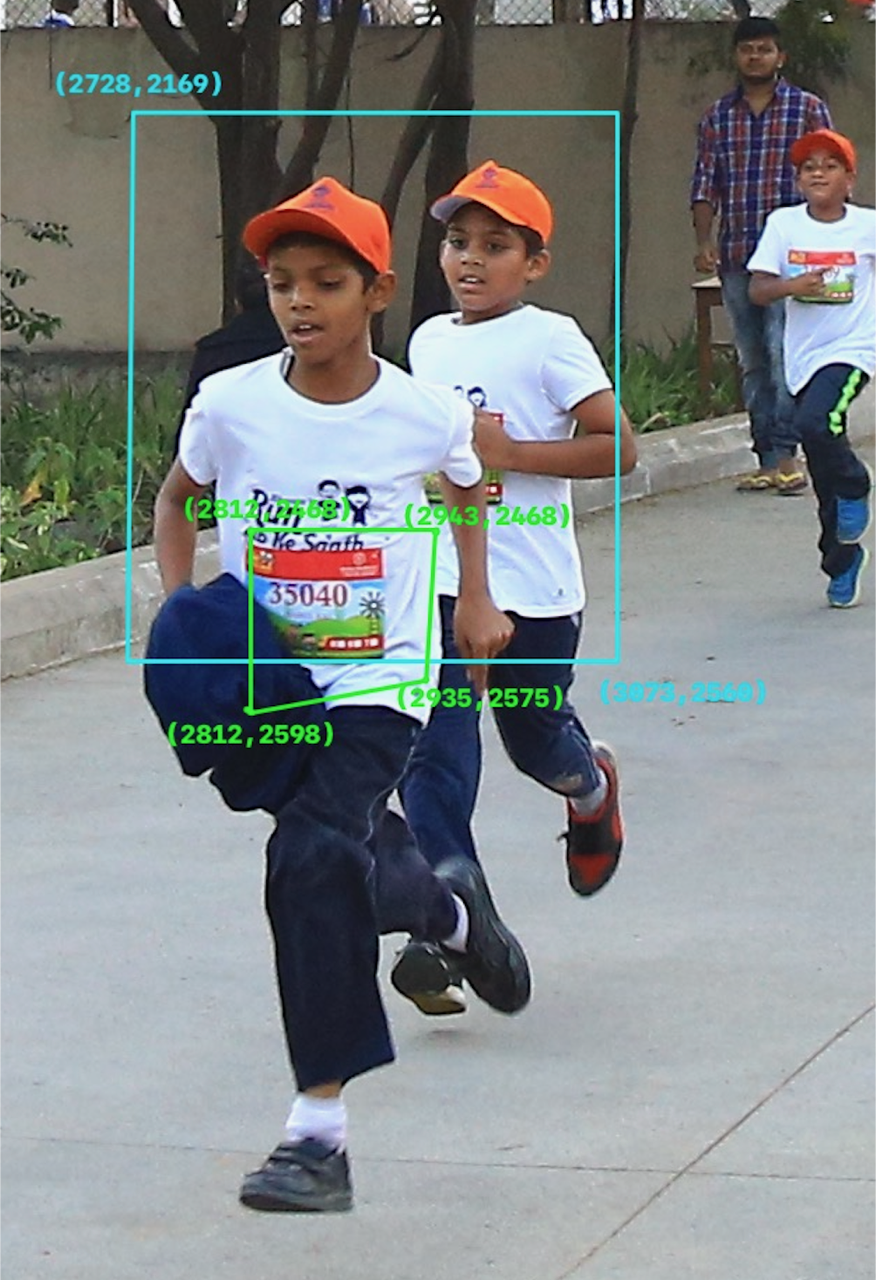
\includegraphics[width=\textwidth]{images/dataset/BadTagging_Overlap}
  \end{subfigure}
  \hspace{\fill}
  \begin{subfigure}[b]{0.3\textwidth}
    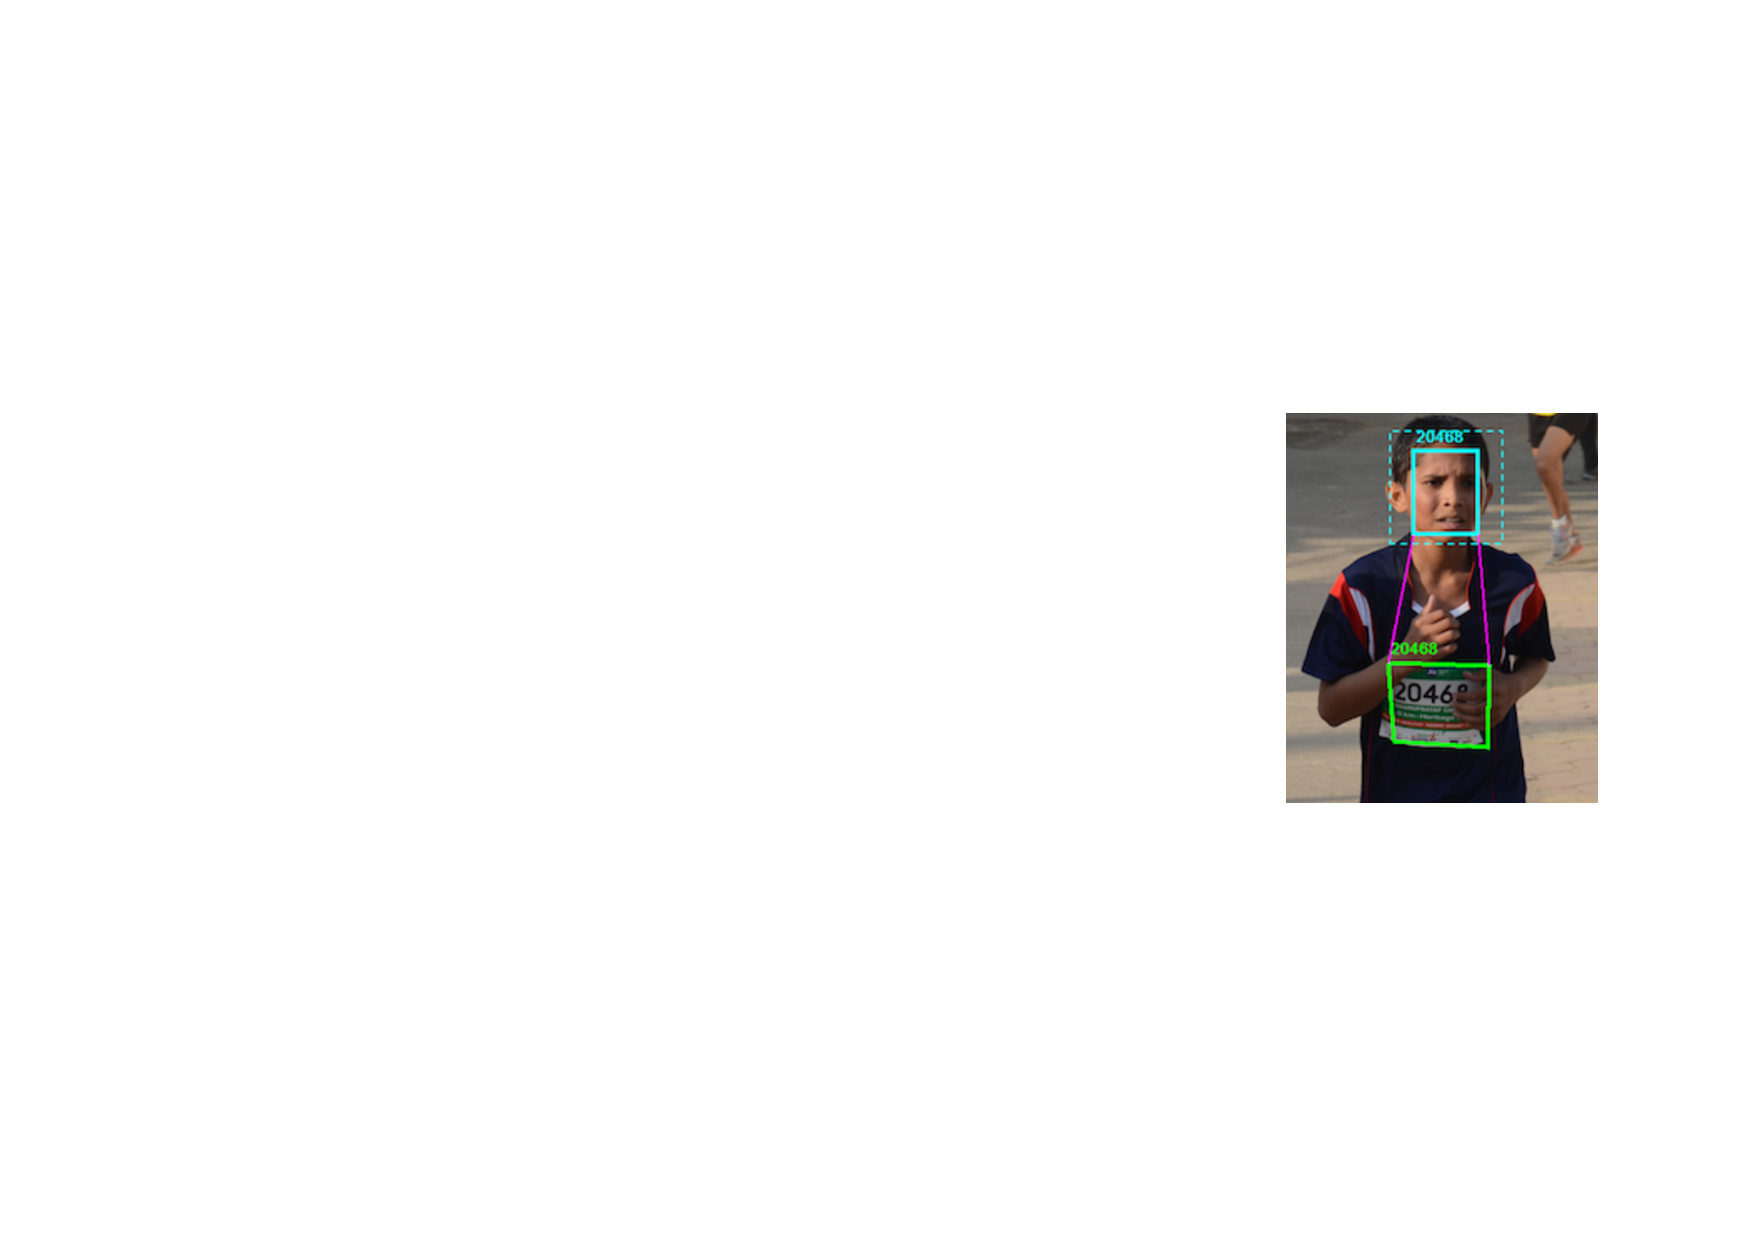
\includegraphics[width=\textwidth]{images/dataset/BadTagging_NotAroundFace}
  \end{subfigure}
  \hspace{\fill}  
  \begin{subfigure}[b]{0.2\textwidth}
    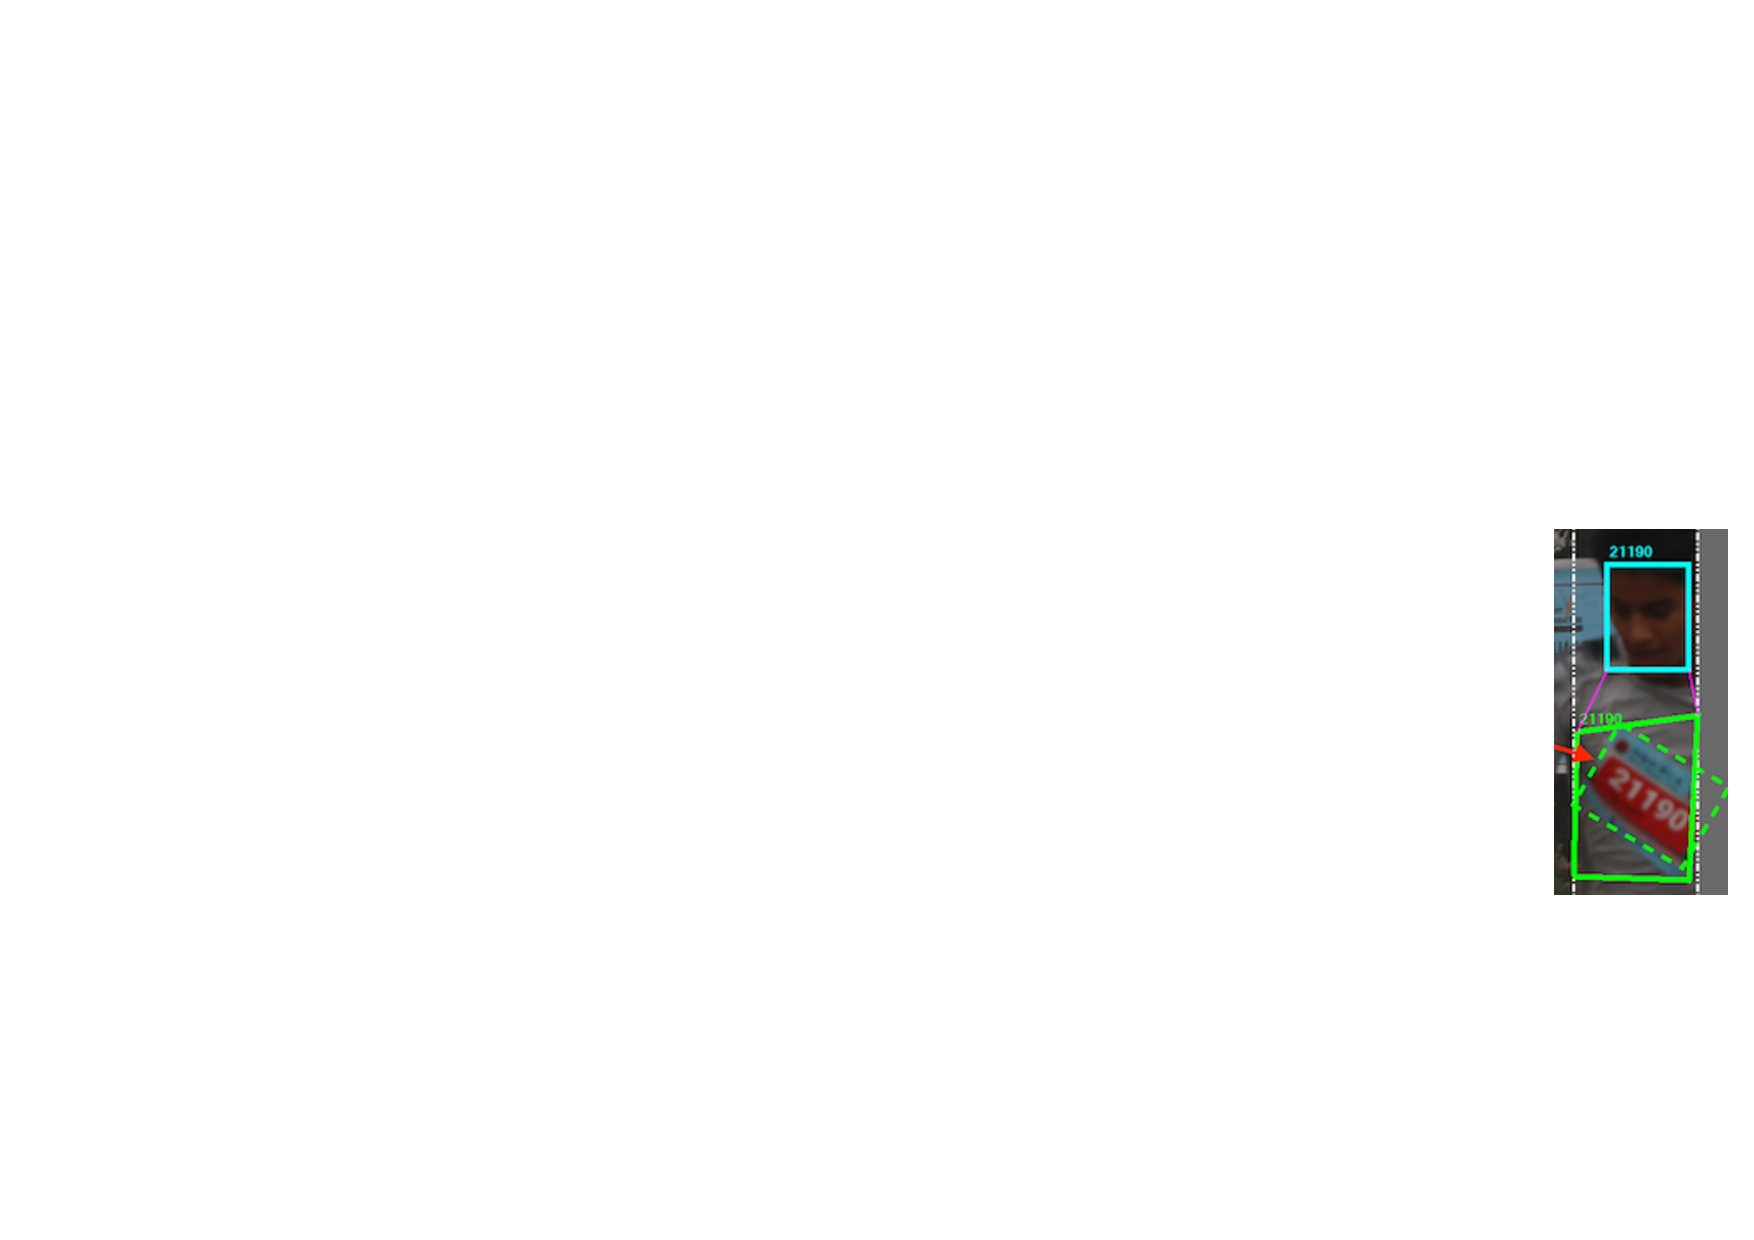
\includegraphics[width=\textwidth]{images/dataset/BadTagging_NotAroundBib}
  \end{subfigure}
  \hspace{\fill}
  
  \caption[Product testing issues identified]{Issues identified from rounds of external testing to the tagging team. Cyan lines indicate face regions, lime lines indicate bib regions, magenta lines indicate bib-to-face guidelines. \textit{Clockwise:} Face region is too far away from bib region; bib region is poorly marked (dotted lines expected); face region is too small (dotted lines expected); face region overlaps bib region.}
  \label{fig:dataset:issues_with_tagging}
\end{figure}

\section{Motivating Case Study: What to Capture?}
\label{sec:dataset:architecture:what_to_capture}

Let us consider the motivating case study of marathon races and determine the model of our dataset. What features do we want to capture from images within our dataset? To answer this question, we need to consider what information we see as relevant in a standard marathon photo (such as \cref{fig:introduction:background:sample_rbns}). We will consider five distinct features in the following sections.

\subsection{Feature 1: Image-Level Features}

There are two features to describe components of the entire photo that we call \textit{Image-level} features:

\begin{enumerate}
  \item whether or not the photo is considered as \textbf{crowded} (\textsc{true} or \textsc{false}), and
  \item an \textit{optional} collection of \textbf{runners} in the photo, given that the photo is not crowded.
\end{enumerate}

\begin{figure}[th]
  \centering
  \begin{subfigure}[b]{0.4\textwidth}
    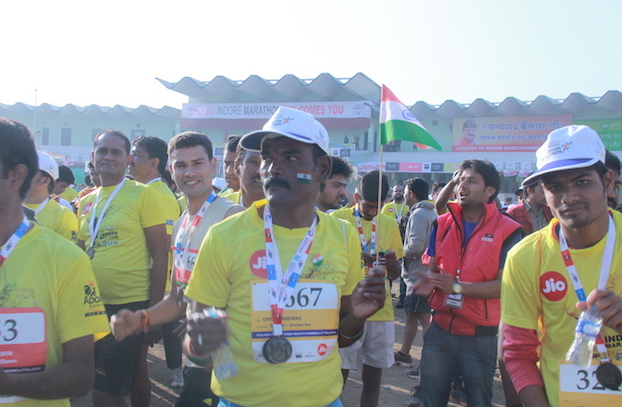
\includegraphics[width=\textwidth]{images/dataset/ImageFeatures_Crowded}
    \caption{\footnotesize A crowded photo.}
    \label{fig:dataset:image_features:crowded}
  \end{subfigure}
  \hspace{0.05\textwidth}
  \begin{subfigure}[b]{0.4\textwidth}
    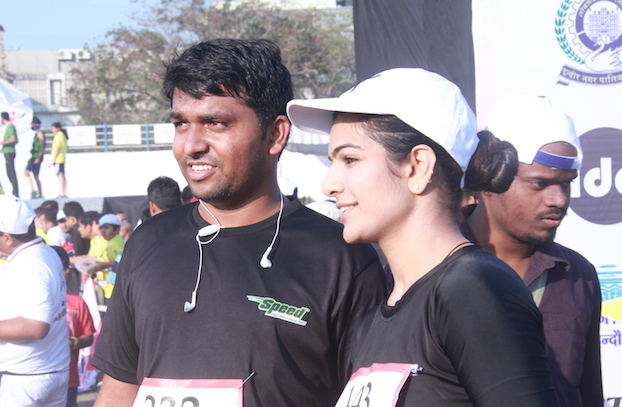
\includegraphics[width=\textwidth]{images/dataset/ImageFeatures_Optional_RBNsCropped}
    \caption{\footnotesize A photo where all \glspl{rbn} are cropped.}
    \label{fig:dataset:image_features:rbns_cropped}
  \end{subfigure}\\
  \vspace{1cm}
  \begin{subfigure}[b]{0.4\textwidth}
    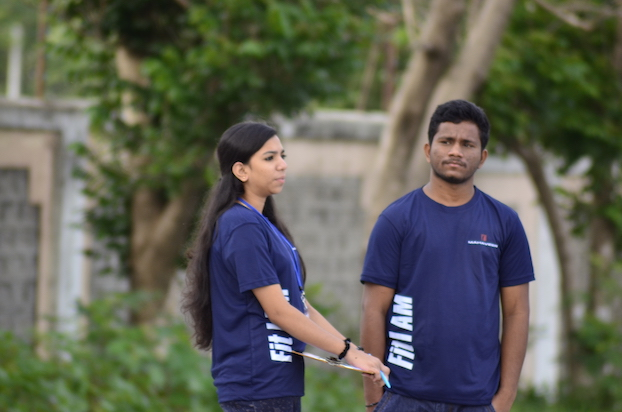
\includegraphics[width=\textwidth]{images/dataset/ImageFeatures_Optional_NoRBNs}
    \caption{\footnotesize A photo where there are no \glspl{rbn} present.}
    \label{fig:dataset:image_features:no_rbns}
  \end{subfigure} 
  \caption[Various image-level features]{Image-level features. In (a), the $PhotoCrowded$ annotation would be marked as \textsc{true}. Note the obstruction of all \glspl{rbn} in this photo. In (b) and (c), $PhotoCrowded$ is \textsc{false}, but there are no $Runners$ to tag.}
  \label{fig:dataset:image_features}
\end{figure}

We train a \gls{nn} based on photos that are not crowded; photos that are considered crowded are typically not desirable as runners prefer photos where they are the key subject. We therefore discard these photos to remove any potential bias tat the \gls{ai} could learn. We can only tag runners on the condition that the photo is not marked as crowded (\cref{fig:dataset:image_features:crowded}). Additionally, in some photos, all \glspl{rbn} are missing within the photo (e.g., hidden behind other runners, cropped out of view) and some photos contain no runners at all (\cref{fig:dataset:image_features:rbns_cropped,fig:dataset:image_features:no_rbns}). We therefore identify this as an \textit{optional} collection as we must associate an \gls{rbn} to a runner---the photo is not crowded, but there are no runners to tag, thereby making the annotation optional. Thus, an \textit{derived attribute} exists with such a collection: the \textit{count} of the runners in a photo is something we can automatically count.

\subsection{Feature 2: Bibs}

We identify the following two annotations of what we would label for a given runner's bib sheet. This is summarised in \cref{fig:dataset:bib_sheet_features}. Within this feature we identify the following annotations for \glspl{rbn}:

\begin{enumerate}
  \item a polygon around the runner's \textbf{bib sheet} that contains the $x$ and $y$ coordinates, given that there are exactly four vertices of this polygon
  \item a string with the runner's \textbf{\gls{rbn}}, once the bib sheet is tagged (exists).
\end{enumerate}

\begin{figure}[p]
  \centering
  \hspace{\fill}
  \begin{subfigure}[b]{0.25\textwidth}
    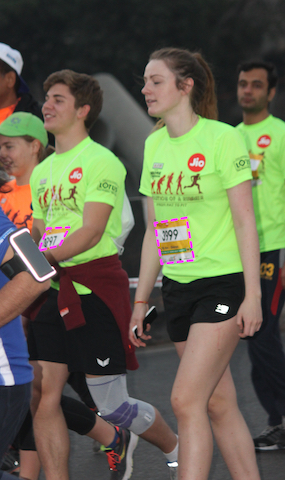
\includegraphics[width=\textwidth]{images/dataset/BibSheet_Detection}
  \end{subfigure}
  \hspace{\fill}
  \begin{subfigure}[b]{0.25\textwidth}
    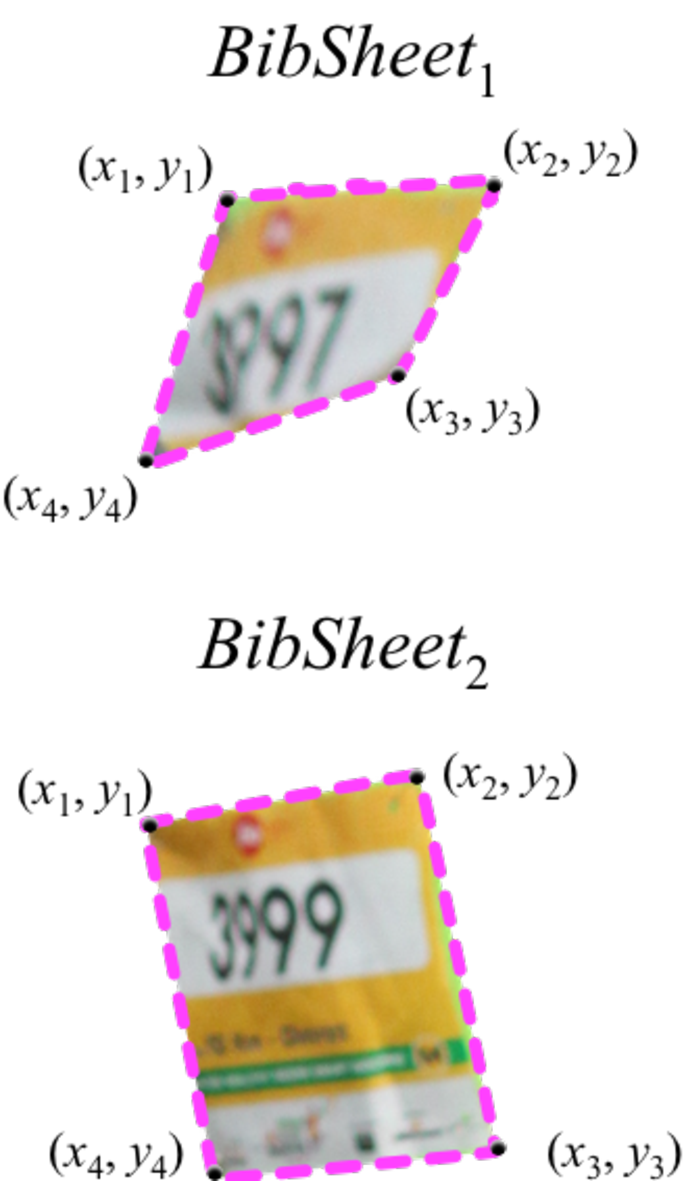
\includegraphics[width=\textwidth]{images/dataset/BibSheet_Area}
  \end{subfigure}
  \begin{subfigure}[b]{0.25\textwidth}
    
\includegraphics[width=\textwidth]{images/dataset/BibSheet_RBN}
  \end{subfigure} 
  \hspace{\fill}
  \caption[Bib Sheet segment-level features]{The bib segment-level feature. \textit{From left to right}: The manually annotated bib sheets in the original photo (outlined in magenta); the relative $BibSheet$ annotations with the four respective vertices; the detected $RBN$ input strings for the corresponding $BibSheet$.}
  \label{fig:dataset:bib_sheet_features}
\end{figure}

\subsection{Feature 3: Faces}

A further feature that is important is the runner's face region (\cref{fig:dataset:face_features}), which could compromise of five annotations:

\begin{enumerate}
  \item a rectangle around the runner's \textbf{face} that contains the two $x$ and $y$ coordinates of the two opposite vertices, given that the $bottom$ of this rectangle are above the $top$ of the bib sheet,
\end{enumerate}

\noindent
and once this face bounds has been tagged, more annotations can be extracted:

\begin{enumerate}
  \setcounter{enumi}{1}
  \item whether or not the runner is \textbf{wearing} a \textbf{hat} (\textsc{true} or \textsc{false}),
  \item whether or not the runner is \textbf{wearing} \textbf{(sun)glasses} (\textsc{true} or \textsc{false}), and
  \item the \textbf{gender} of the runner (\textsc{male}, \textsc{female}, or \textsc{unsure}).
\end{enumerate}

The bib sheet polygon would contain four \textit{explicit attributes} required as input by the tagger: the coordinates of its four vertices, $\{ (x_{1}, y_{1}), (x_{2}, y_{2}), (x_{3}, y_{3}), (x_{4}, y_{4}) \}$. Similarly, there are two explicit attributes required for the runner's face rectangle: the coordinates of the top left and the bottom right of the rectangle (i.e., the two opposite vertices) of the runner's face bounds, $\{ (x_{1}, y_{1}), (x_{2}, y_{2}) \}$. As both of these are shapes, we can automatically calculate the derived attributes from these coordinates:  $\{ top, left, bottom, right, width, height \}$.

\begin{figure}[p]
  \centering
  \hspace{\fill}
  \begin{subfigure}[b]{0.25\textwidth}
    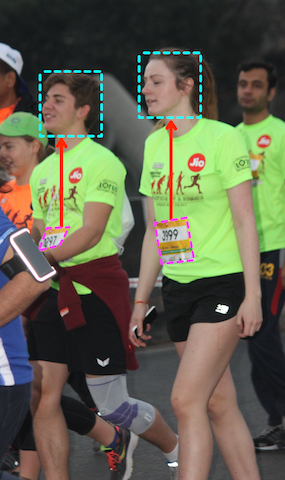
\includegraphics[width=\textwidth]{images/dataset/FaceBounds_Detection}
  \end{subfigure}
  \hspace{\fill}
  \begin{subfigure}[b]{0.25\textwidth}
    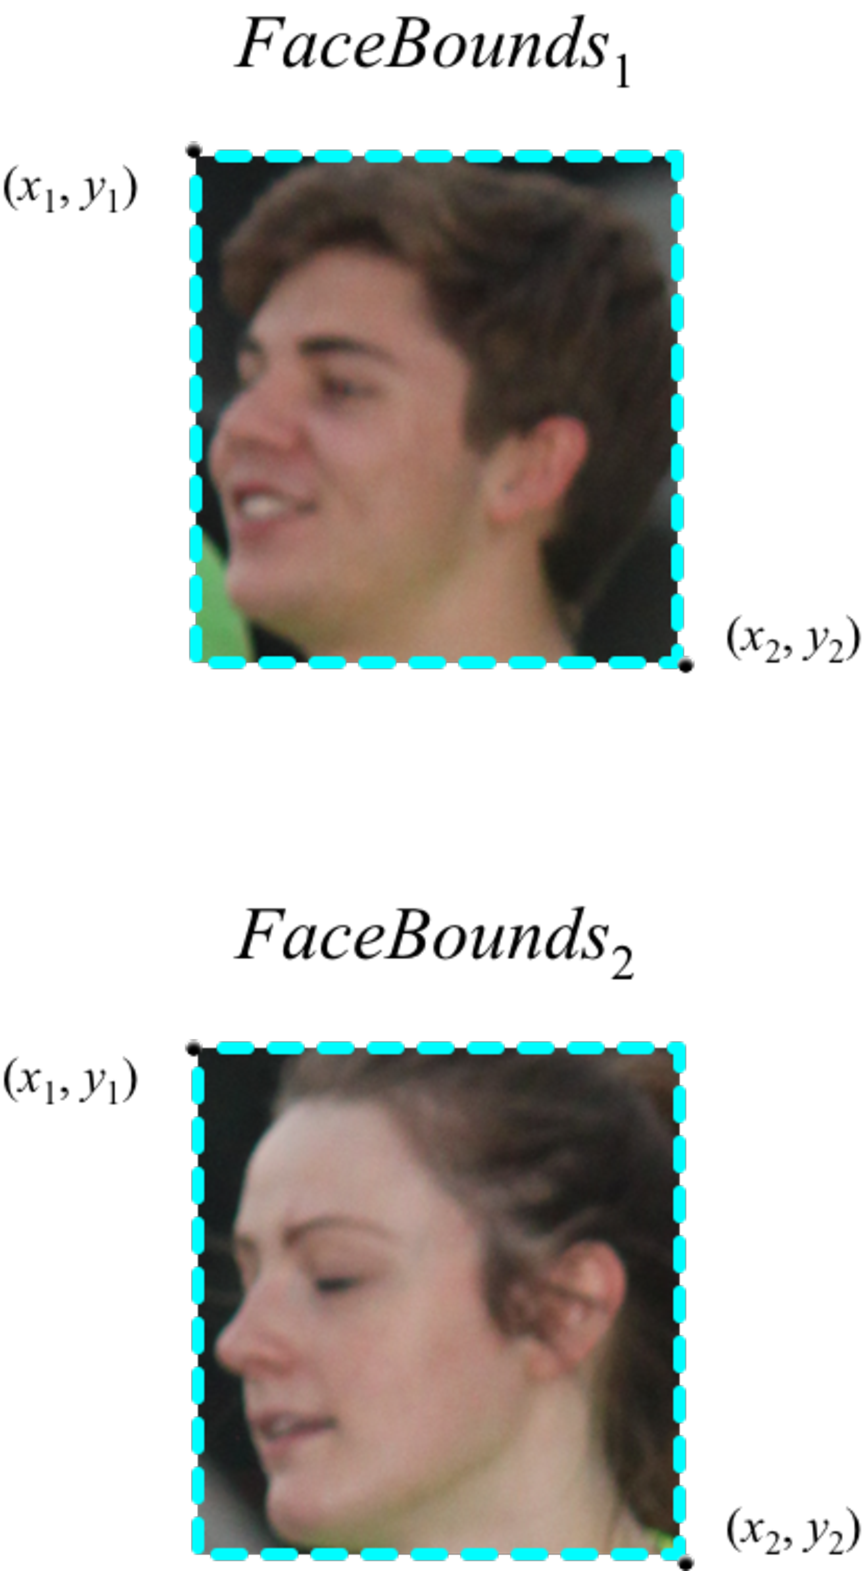
\includegraphics[width=\textwidth]{images/dataset/FaceBounds_Area}
  \end{subfigure}
  \hspace{\fill}
  \caption[Face Bounds segment-level features]{The face segment-level feature. \textit{Left}: The manually tagged face regions (cyan) that comply with the conditions that the bottom must be above the top of the bib (red arrows). \textit{Right}: the relative $FaceBounds$ annotations with the two opposite vertices. Other annotations in this feature would be: $WearingHat{1,2} = WearingGlasses{1,2} = \textsc{false}$, $Gender_{1} = \textsc{male}$, $Gender_{2} = \textsc{female}$.}
  \label{fig:dataset:face_features}
\end{figure}

%Given that the face region is tagged, we can then annotate:
%
%\begin{enumerate}
%  \item the `base classifications' of the person, and
%  \item the `colour classifications' of the person.
%\end{enumerate}

\subsection{Feature 4: Prominence}

We can now identify another feature, the prominence of the runner within the photo. These would consist of three annotations:

\begin{enumerate}
  \item whether or not the runner's \textbf{face} is \textbf{visible} (\textsc{true} or \textsc{false}),
  \item whether or not the runner is \textbf{blurry} (\textsc{true} or \textsc{false}),
  \item the \textbf{\gls{lop}} that the runner buys the photo (\textsc{no}, \textsc{maybe}, \textsc{yes}),
\end{enumerate}

A runner's face is considered `invisible' if it is obstructed by another object, cropped out of the image, or if the runner is looking down. See \cref{fig:dataset:face_prominence}. Runners are more likely purchase a photo if they are looking at the camera, and likewise if they are blurry in the image; these therefore have a significant impact on their prominence. We also define the \glsx{lop} value as a qualitative metric. We ask the data tagger to `picture' themselves as runner, and if so, we ask if they would purchase it. We then use this metric to train positive samples of good photos (\gls{lop} = \textsc{yes}) and samples of bad photos (\gls{lop} = \textsc{no}). Where \textsc{maybe} is provided, the runner is ignored to prevent training the network with indeterminate samples. Refer to \cref{fig:dataset:lop_prominence} for examples of the varying \gls{lop} values. 

\begin{figure}[p]
  \centering
  \hspace{\fill}
  \begin{subfigure}[b]{0.25\textwidth}
    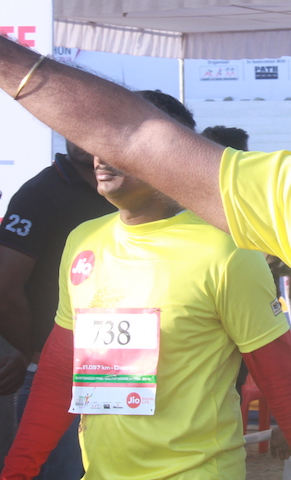
\includegraphics[width=\textwidth]{images/dataset/Prominence_FaceNotVisible_Covered}
    \caption{Face obstructed}
  \end{subfigure}
  \hspace{\fill}
  \begin{subfigure}[b]{0.25\textwidth}
    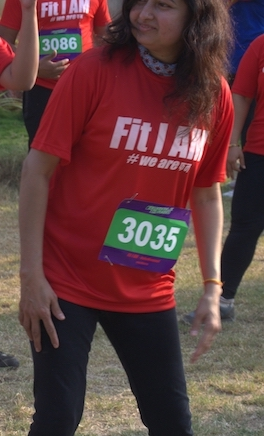
\includegraphics[width=\textwidth]{images/dataset/Prominence_FaceNotVisible_Cropped}
      \caption{Face cropped}
  \end{subfigure}
  \hspace{\fill}
  \begin{subfigure}[b]{0.25\textwidth}
    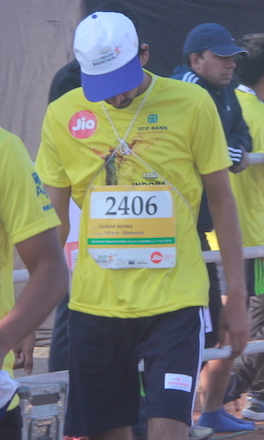
\includegraphics[width=\textwidth]{images/dataset/Prominence_FaceNotVisible_LookingDown}
    \caption{Face looking down}
  \end{subfigure}
  \hspace{\fill}
  \caption[Face visibility and its effect on prominence]{The $FaceVisible$ plays a significant impact on the prominence feature. Above are cases where the face would be marked as not visible.}
  \label{fig:dataset:face_prominence}
\end{figure}

\begin{figure}[p]
  \centering
  \hspace{\fill}
  \begin{subfigure}[b]{0.25\textwidth}
    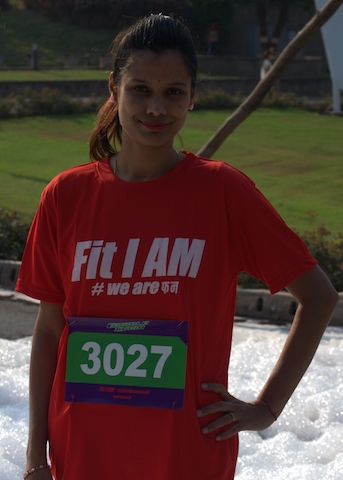
\includegraphics[width=\textwidth]{images/dataset/Prominence_LoP_Yes}
    \caption{\gls{lop} = \textsc{yes}}
  \end{subfigure}
  \hspace{\fill}
  \begin{subfigure}[b]{0.25\textwidth}
    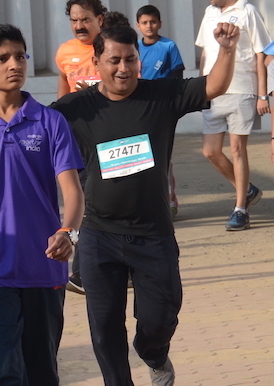
\includegraphics[width=\textwidth]{images/dataset/Prominence_LoP_Maybe}
    \caption{\gls{lop} = \textsc{maybe}}
  \end{subfigure}
  \hspace{\fill}
  \begin{subfigure}[b]{0.25\textwidth}
    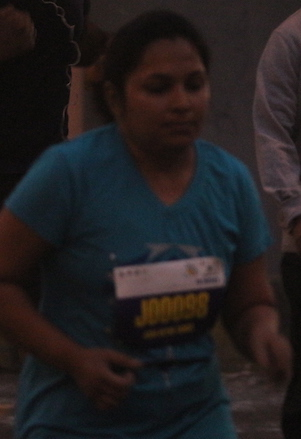
\includegraphics[width=\textwidth]{images/dataset/Prominence_LoP_No}
    \caption{\gls{lop} = \textsc{no}}
  \end{subfigure}
  \hspace{\fill}
  \caption[Variant Purchase Likelihoods]{Various examples of the $\gls{lop}$ values. In (a), the woman is clearly posing and is the primary subject of the photo. In (b), the runner is in focus in a pose, but is behind another runner and there are other runners behind him. In (c), the woman is out of focus, is blurry, and this photo has very poor lighting conditions.}
  \label{fig:dataset:lop_prominence}
\end{figure}

\subsection{Feature 5: Colours}

Another feature we can capture is a way to identify runners by the colour of their clothing. (Within our dataset, various clothing items of distinct colours are given to runners for particular races.) These features comprise of four annotations:

\begin{enumerate}
  \item an \textit{optional} \textbf{colour} of the runner's \textbf{hat}, given that they were annotated as wearing a hat,
  \item the \textbf{colour} of the runner's \textbf{shirt},
  \item an \textit{optional} \textbf{colour} of the runner's \textbf{shorts}, and
  \item an \textit{optional} \textbf{colour} of the runner's \textbf{shoes}.
\end{enumerate}

% TODO: Example of colour matching. Do we capture the coordinates?

The colour of a runner's shirt is required, as we expect that a bib would be detected on the shirt of a runner (which would be tagged). The other colour annotations are all optional, as it is likely that some of these clothing items may be cropped out of the photo or is not visible. Furthermore, the hat colour can only be specified on the condition that the tagger has marked the runner has wearing a hat.

We can segment groups of the annotations we extract into features of two categories: annotations that feature at the \textit{image}-level and those that do not, which we call \textit{segment}-level features. The image-level features are those which apply to the entire image (i.e., $PhotoCrowded$, $Runners$). Those that apply at the segment level can be grouped into what types of features we are extracting: the runner's bib, face, their prominence and their colour identification.

In summary, we have identified a total of 5 features of 15 annotations, which are summarised within \cref{tab:dataset:annotation_summary}. Each of these annotations can be classified with a name and type, conditions for the annotation to be valid, dependencies on other annotations to exist before the annotation can be made, explicit attributes which the tagger must specify, derived attributes which we can automatically compute, possible values which limit the range of data for that annotation, and whether or not the annotation is optional.

\begin{landscape}

\begin{table}[p]
  \centering
  \caption[Summary of annotations captured in the dataset]{\centering A summary of the annotations we wish to capture from our dataset. Image and segment-level features are separated using the double line.}
  \label{tab:dataset:annotation_summary}
  \tablefitlandscape{
    \begin{tabular}{llllllllll}
      \toprule
        \textbf{Feature} &
        \textbf{Annotation} &
        \textbf{Type} &
        \textbf{Conditions} &
        \textbf{Dependencies} &
        \textbf{Explicit Attributes} &
        \textbf{Derived Attributes} &
        \textbf{Possible Values} &
        \textbf{Default} &
        \textbf{Optional}
      \\
      \midrule
        \multirow{2}{*}{Image-Level} &
        $PhotoCrowded$ &
        Boolean &
        N/A &
        N/A &
        N/A &
        N/A &
        $\{ \textsc{true}, \textsc{false} \}$&
        \textsc{false} &
        No
      \\
        &
        $Runners$ &
        Collection &
        $\{ PhotoCrowded = \textsc{false} \}$ &
        N/A &
        N/A &
        $\{count\}$ &
        N/A &
        \textsc{null} &
        Yes
      \\
      \midrule
      \midrule
        \multirow{2}{*}{Bib} &
        $BibSheet$ &
        Polygon &
        $\{ vertices = 4 \}$ &
        N/A &
        $\{ x_{1} \dots x_{4}, y_{1} \dots y_{4} \}$ &
        $\{ top, left, bottom, right, width, height \}$ &
        N/A &
        \textsc{null} &
        No
      \\
        &
        $\gls{rbn}$ &
        Label &
        N/A &
        $BibSheet$ &
        N/A &
        N/A &
        N/A &
        \textsc{null} &
        No
      \\
      \midrule
        \multirow{2}{*}{Face} &
        $FaceBounds$ &
        Rectangle &
        $\{ bottom > BibSheet_{top} \}$  &
        $BibSheet$ &
        $\{ x_{1}, y_{1}, x_{2}, y_{2}\}$ &
        $\{ top, left, bottom, right, width, height \}$ &
        N/A &
        \textsc{null} &
        No
      \\
        &
        $WearingHat$ &
        Boolean &
        N/A &
        $FaceBounds$ &
        N/A &
        N/A &
        $\{ \textsc{true}, \textsc{false} \}$&
        \textsc{false} &
        No
      \\
        &
        $WearingGlasses$ &
        Boolean &
        N/A &
        $FaceBounds$ &
        N/A &
        N/A &
        $\{ \textsc{true}, \textsc{false} \}$&
        \textsc{false} &
        No
      \\
        &
        $Gender$ &
        Category &
        N/A &
        $FaceBounds$ &
        N/A &
        N/A &
        $\{ \textsc{male}, \textsc{female}, \textsc{unsure} \} $ &
        \textsc{male} &
        No
      \\
      \midrule
        \multirow{2}{*}{Prominence} &
        $\gls{lop}$ &
        Category &
        N/A &
        $FaceBounds$ &
        N/A &
        N/A &
        $\{ \textsc{no}, \textsc{maybe}, \textsc{yes} \}$ &
        \textsc{maybe} &
        No
      \\
        &
        $FaceVisible$ &
        Boolean &
        N/A &
        $FaceBounds$ &
        N/A &
        N/A &
        $\{ \textsc{true}, \textsc{false} \}$&
        \textsc{true} &
        No
      \\
        &
        $Blurry$ &
        Boolean &
        N/A &
        $FaceBounds$ &
        N/A &
        N/A &
        $\{ \textsc{true}, \textsc{false} \}$&
        \textsc{false} &
        No
      \\
      \midrule
        \multirow{2}{*}{Colours} &
        $ShirtColor$ &
        Color &
        N/A &
        $FaceBounds$ &
        $\{ red, green, blue \}$ &
        N/A &
        N/A &
        \textsc{null} &
        No
      \\
        &
        $ShoeColor$ &
        Color &
        N/A &
        $FaceBounds$ &
        $\{ red, green, blue \}$ &
        N/A &
        N/A &
        \textsc{null} &
        Yes
      \\
        &
        $ShortsColor$ &
        Color &
        N/A &
        $FaceBounds$ &
        $\{ red, green, blue \}$ &
        N/A &
        N/A &
        \textsc{null} &
        Yes
      \\
        &
        $HatColor$ &
        Color &
        $\{ WearingHat = \textsc{true} \}$ &
        $FaceBounds$ &
        $\{ red, green, blue \}$ &
        N/A &
        N/A &
        \textsc{null} &
        Yes
      \\
      \bottomrule
    \end{tabular}
  }
\end{table}

\end{landscape}

% Run through an example of what it is we need to capture for our study & why (Refer to meeting 1 notes).
% state diagram of things we need to classify (break down diagram).

\section{Describing the Metamodel}
\label{sec:dataset:architecture:metamodel}

% Conceptualise what we have in our workflow as a meta model.
% What are the components, and constraints? Discuss why we needed to add in constraints... Feedback from India

In the example given in \cref{tab:dataset:annotation_summary}, we describe a model which was derived using information discovered from Argus' incremental development. In this section, we generalise this information and develop a metamodel . This metamodel is represented as a \gls{uml} class diagram, shown in \cref{fig:dataset:metamodel_class_diagram}.

\begin{figure}[h]
  \centering
  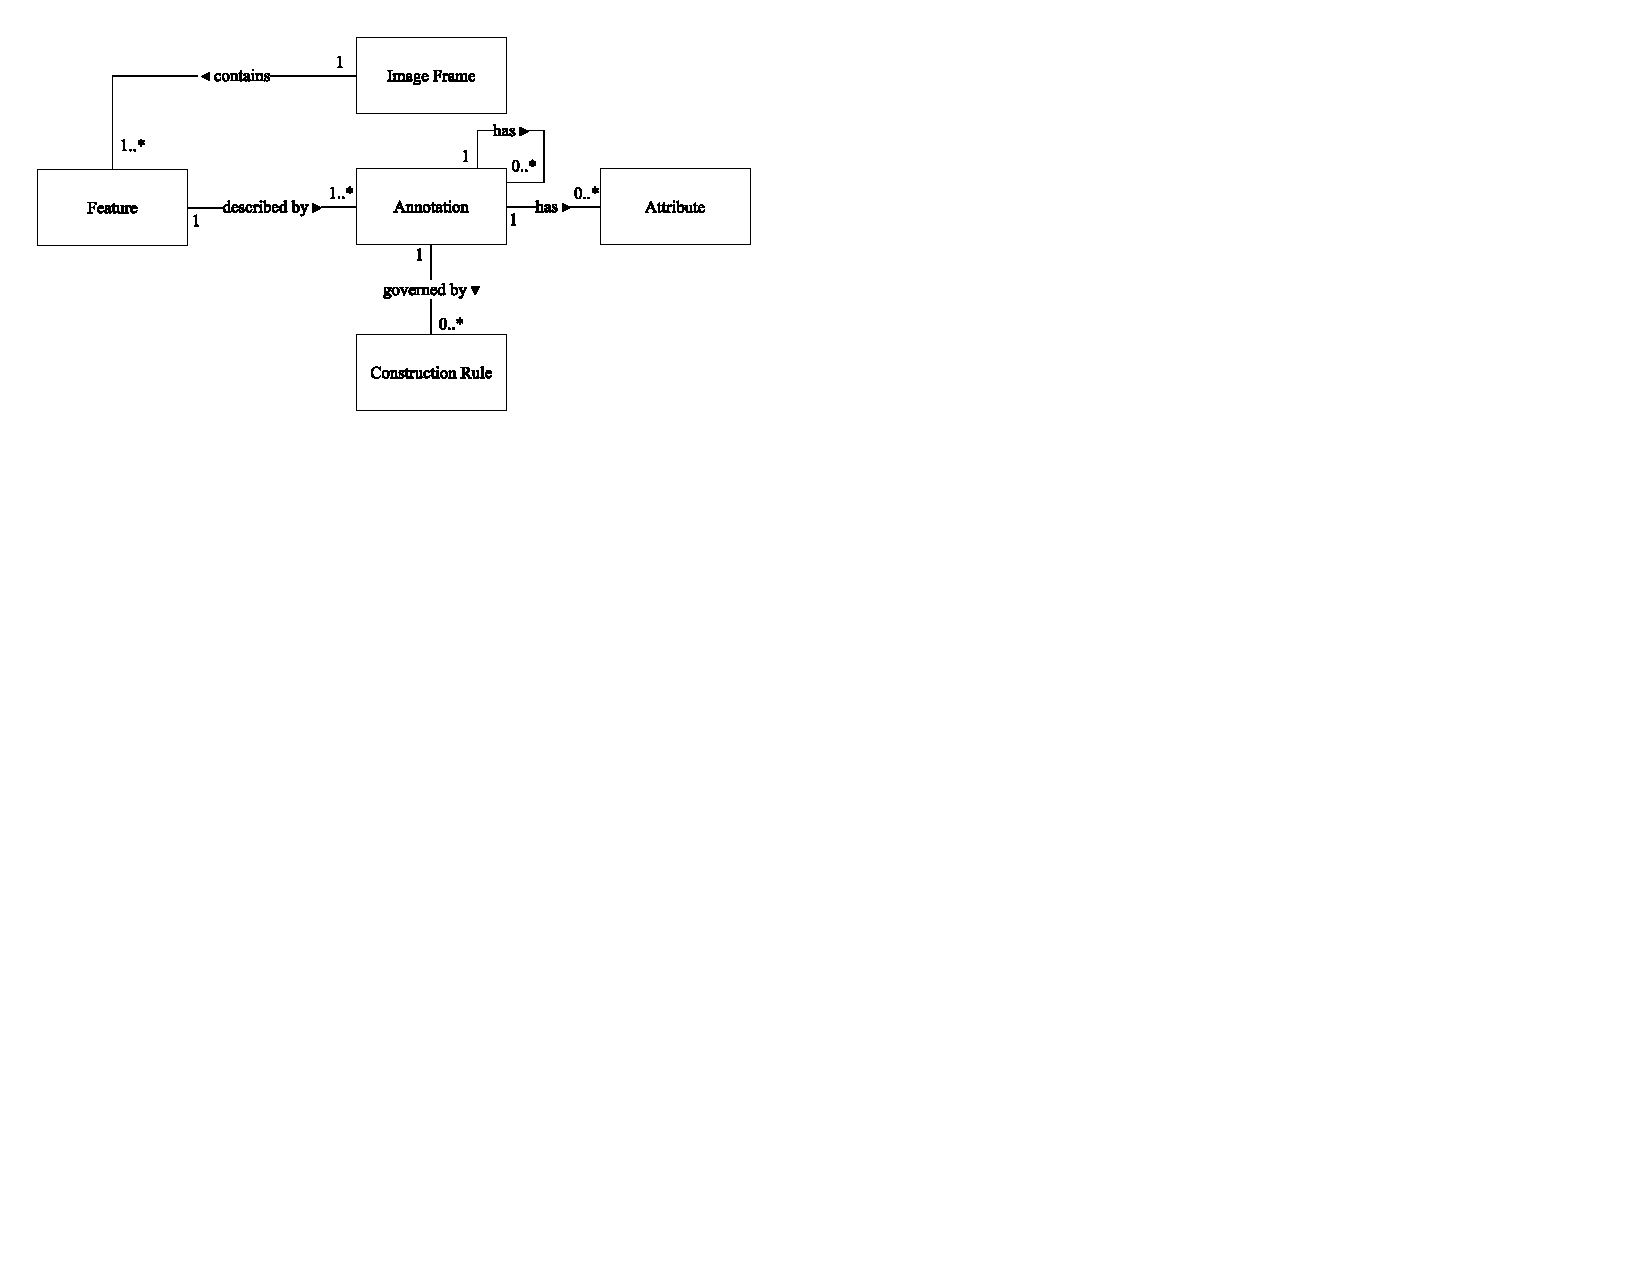
\includegraphics[width=\textwidth]{images/dataset/metamodel_class_diagram}
  \caption[Class diagram of our proposed metamodel]{A class diagram of our proposed metamodel.}
  \label{fig:dataset:metamodel_class_diagram}
\end{figure}

The core concept of this metamodel is an \textit{Annotation}, which (collectively) describe a feature within an image. Annotations may contain additional attributes to further extend what information they contain, and are governed by a set constrictions that we call \textit{Construction Rules}.

These form layers of data within images that we annotate, which can be represented in a hierarchical data format (e.g., a tree) that describes the layering of a fully annotated photo's features. These classes have further depth that are captured via inheritance models, presented in \cref{ch:metamodel_class_diagrams}.

We describe each of these classes in the following sections.

\subsection{Image Frame}

An image frame is any visual representation of a graphic. We extend the possibilities of our metamodel beyond just static images---these frames may be those found in videos also.

\subsection{Feature}

Image frames contain a certain number of features. These features are the key `concepts' within the image that we want to capture. There are two main features: (1) image-level features, and (2) segment-level features. Image-level features are those that apply to the entire frame and do not exist in a broken down context---we can't break down these features into their own subjects. This contrasts to segment-level features, which are features that only apply to a segmented region of the image. We identified four segment-level features in our example (all of which relate to one runner): Bib, Face, Prominence and Colours.

\subsection{Annotation}

Annotations are a set of feature descriptors that describes what the feature is compromised of. From \cref{tab:dataset:annotation_summary}, we describe a simple type system consisting of the following: \textit{Boolean}s, a restricted form of the \textit{Category} type (where possible values are $\{ \textsc{true}, \textsc{false} \}$); \textit{Polygon}s and \textit{Rectangle}s, generalised into a high-level \textit{Boundary} type; and \textit{Colour}s, represented as an RGB represented hexadecimal \textit{Label} (a generic labelling type). This only leaves our \textit{Collection} of runners: a data type which encompasses multiple annotations. Attributes can therefore be described by a type system that is generalisable from \textit{Labels}, \textit{Boundaries}, \textit{Collections} and \textit{Categories}. We model this as a type tree (\cref{fig:metamodel_class_diagrams:annotation}).

\subsection{Construction Rules} 

Construction Rules govern how attributes can be made. We break these down into four types: Dependencies, Conditions, Optionality and Restrictions (\cref{fig:metamodel_class_diagrams:construction_rules}). Some annotations are dependent on others existing---these are rules that we name \textit{Dependencies}. For instance, we cannot annotate an \gls{rbn} if there is no $BibSheet$ annotated. Likewise, a $FaceBounds$ is dependent on where the $BibSheet$ is, and so the $BibSheet$ must be marked up first. These dependencies add order in which features are being extracted, which is important to the tagger marking up the photo. A \textit{Condition} is a construction rule that disallows a data tagger to create an annotation until a condition is met by the annotator. For instance, we can never have a $BibSheet$ above a $FaceBounds$, so when we can specify this as a condition. These are not bound to just geometric constraints; we also see that we cannot tag $Runners$ if the $PhotoCrowded$ annotation is marked as \textsc{true}. Not all annotations are needed---in these cases the annotation is restricted by an \textit{Optional} construction rule; by default, all annotations are required, but we can specify these to be optional using such a rule. Lastly, \textit{Restrictions} exist to prevent invalid data from being tagged. In our example, we implemented two restrictions in Argus: (1) a face region must be tagged within an aspect ratio of $3 \times BibSheet_{width} : 5 \times BibSheet_{height}$, and (2) the opposite edges of a face region must be at least 15 pixels apart. This helps prevent issues shown in \cref{fig:dataset:issues_with_tagging}.

\begin{figure}[p]
  \centering
  
  \begin{subfigure}[b]{0.8\textwidth}
    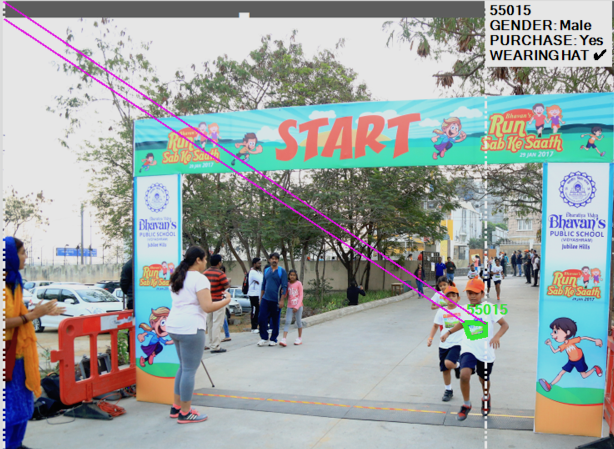
\includegraphics[width=\textwidth]{images/dataset/BadTagging_TooFar}
  \end{subfigure}\\
  \vspace{1cm}
  \hspace{\fill}
  \begin{subfigure}[b]{0.3\textwidth}
    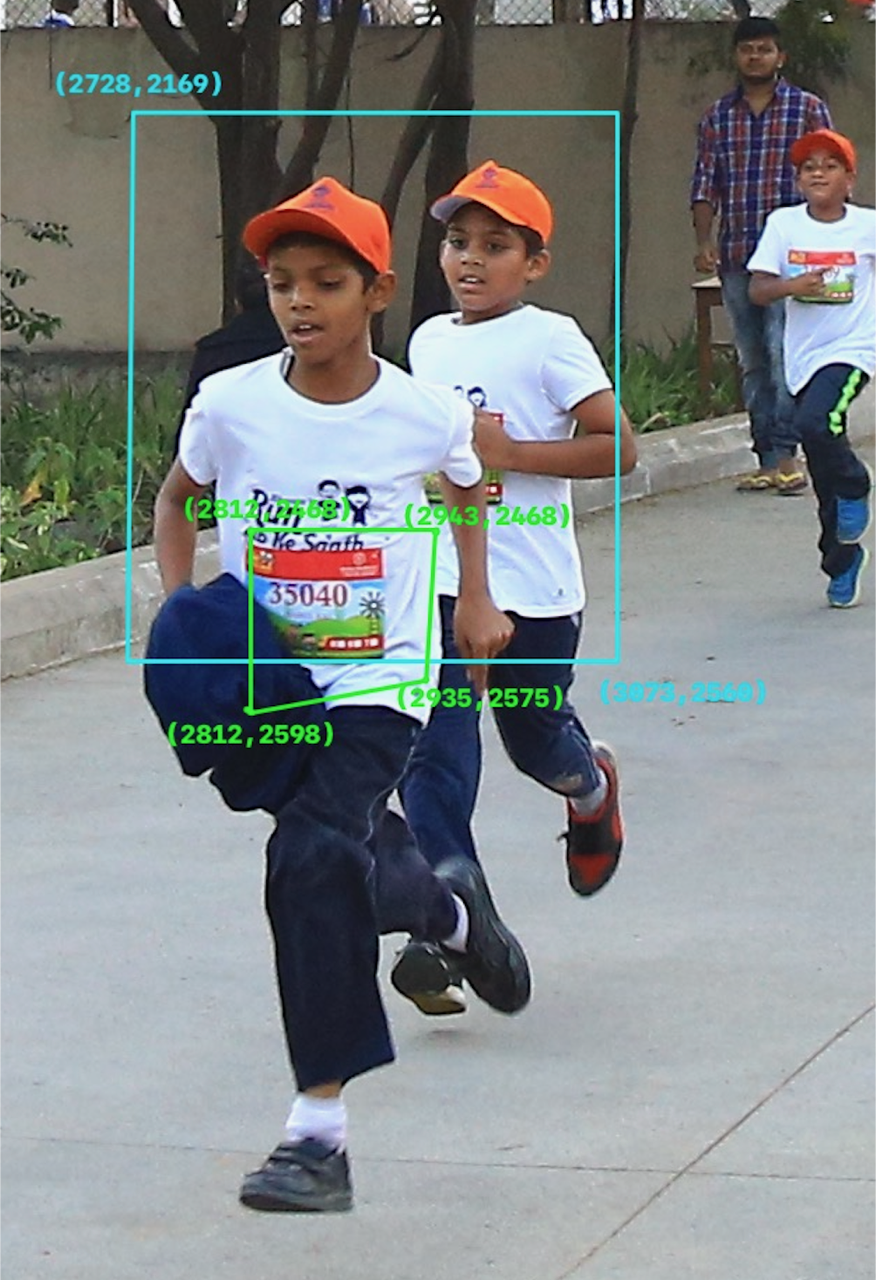
\includegraphics[width=\textwidth]{images/dataset/BadTagging_Overlap}
  \end{subfigure}
  \hspace{\fill}
  \begin{subfigure}[b]{0.3\textwidth}
    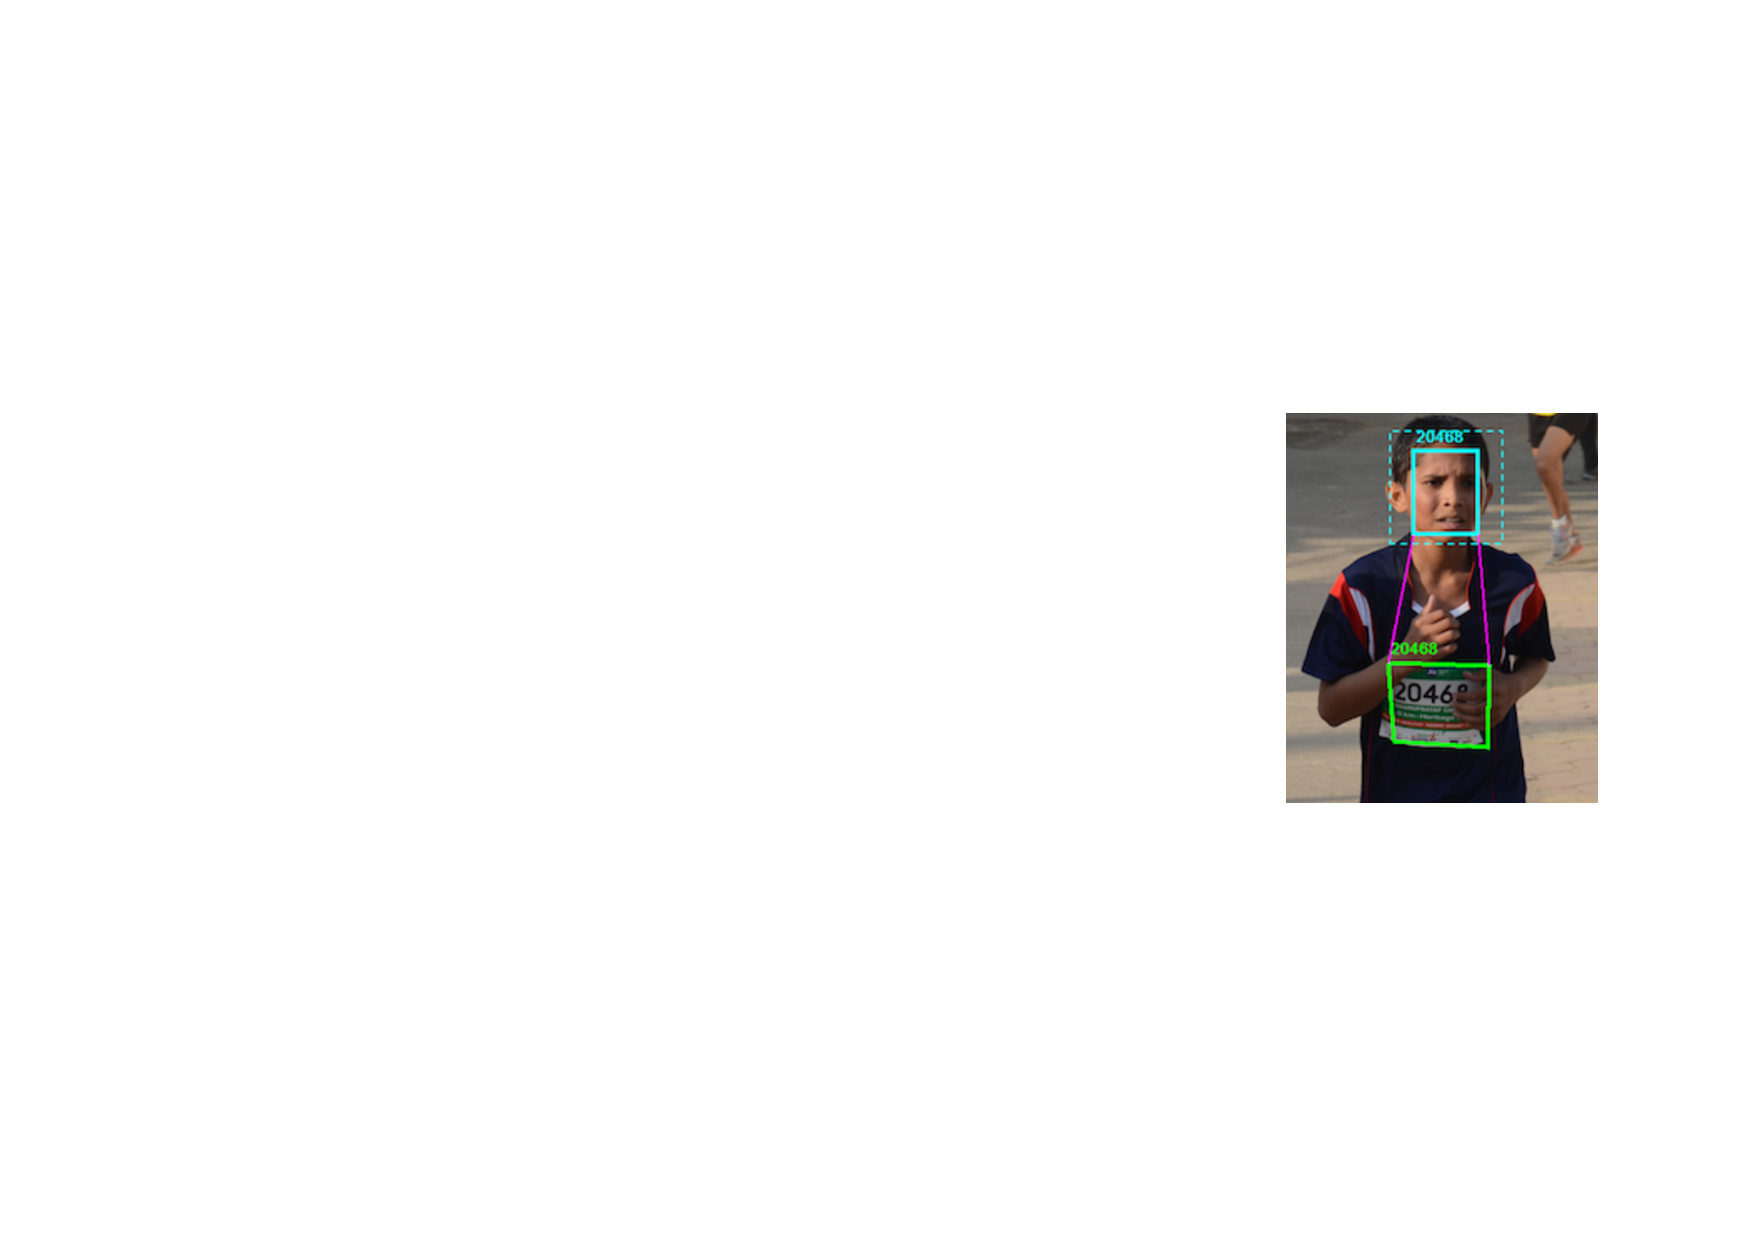
\includegraphics[width=\textwidth]{images/dataset/BadTagging_NotAroundFace}
  \end{subfigure}
  \hspace{\fill}  
  \begin{subfigure}[b]{0.2\textwidth}
    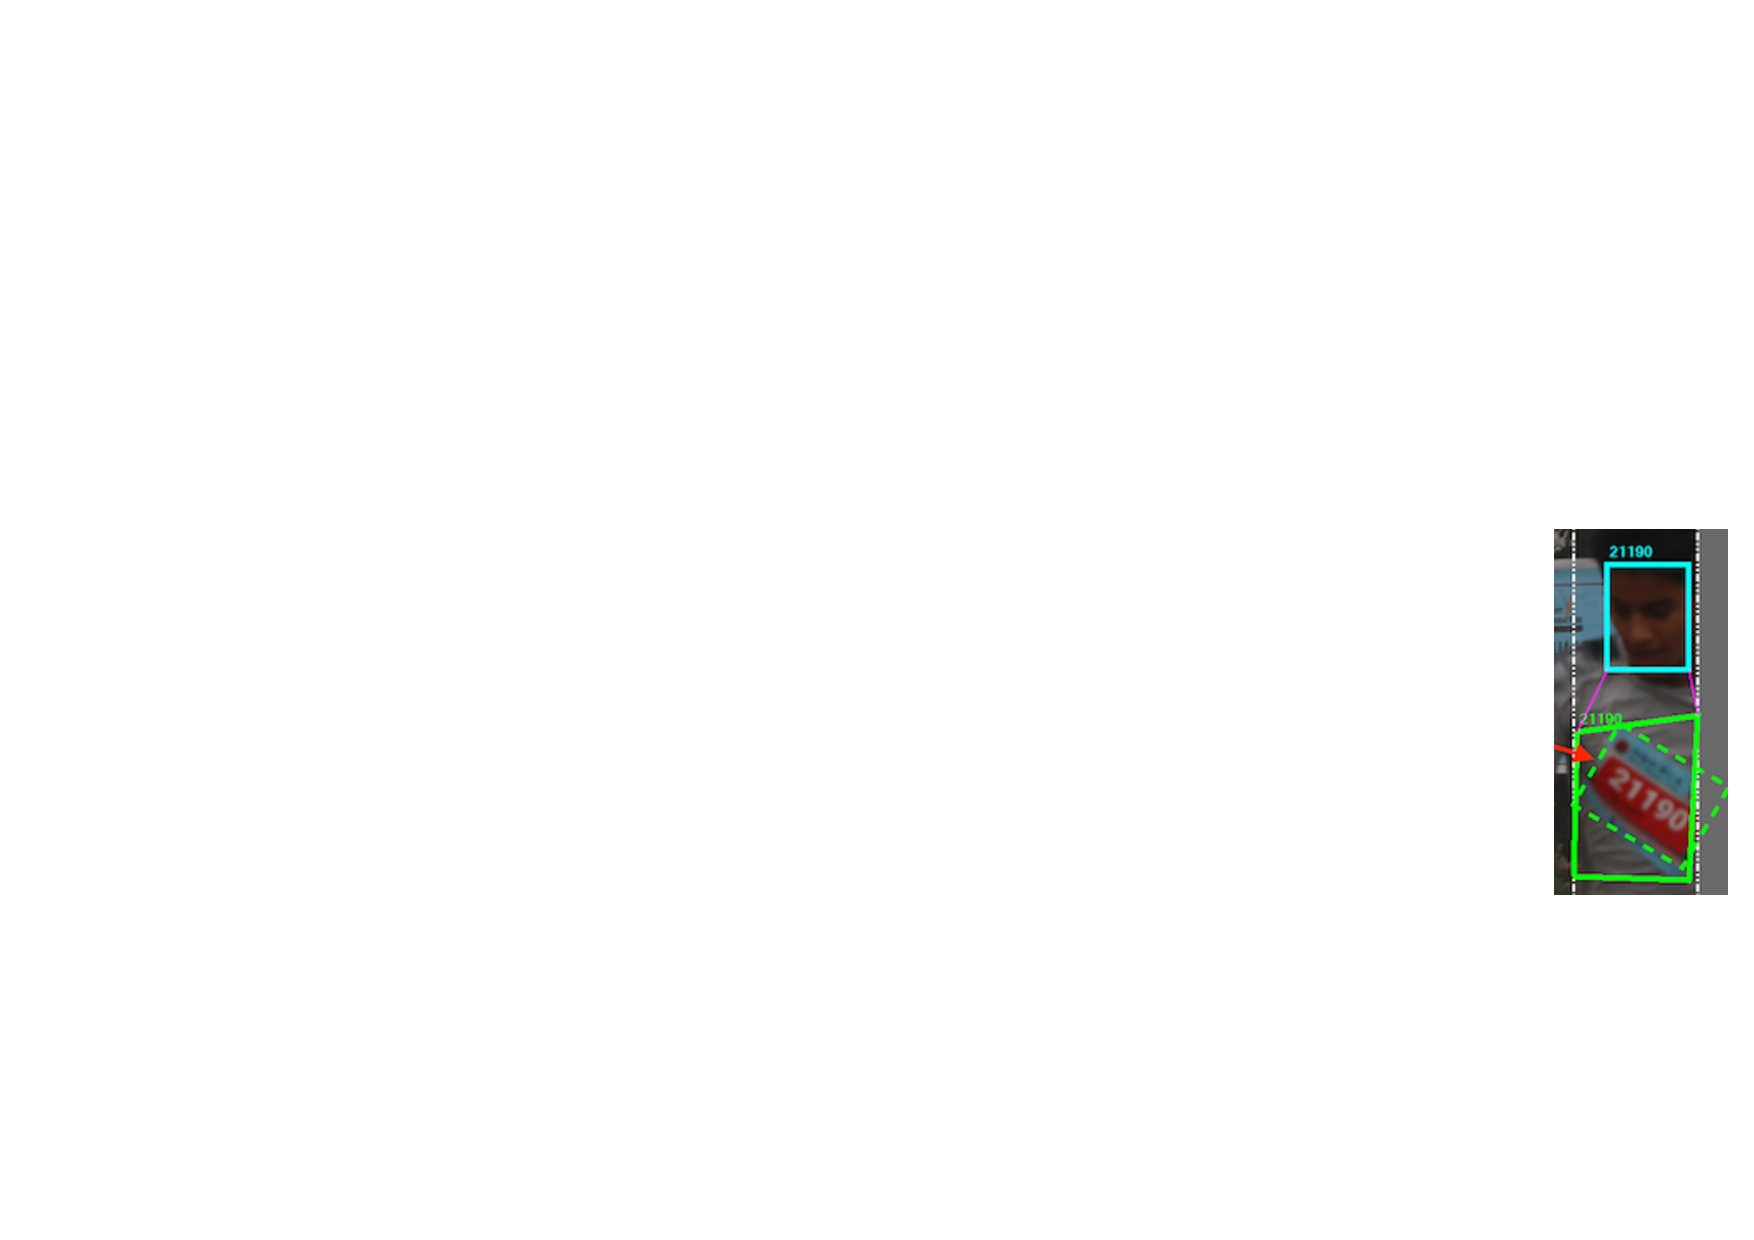
\includegraphics[width=\textwidth]{images/dataset/BadTagging_NotAroundBib}
  \end{subfigure}
  \hspace{\fill}
  
  \caption[Product testing issues identified]{Issues identified from rounds of external testing to the tagging team. Cyan lines indicate face regions, lime lines indicate bib regions, magenta lines indicate bib-to-face guidelines. \textit{Clockwise:} Face region is too far away from bib region; bib region is poorly marked (dotted lines expected); face region is too small (dotted lines expected); face region overlaps bib region.}
  \label{fig:dataset:issues_with_tagging}
\end{figure}

\subsection{Attributes}

Attributes exist as a means to capture further information about an annotation. We represent attributes in our metamodel as either derived or explicit. As stated in \cref{sec:dataset:architecture:what_to_capture}, those attributes which are required for the tagger to manually markup are explicit (i.e., manually must be added) whereas those that can be computed by the system are derived (i.e., inferred from explicit attributes). A useful example of derived attributes may be the bounding box and area that inferred from a polygon, both of which are key values required in training \glspl{nn}.

\section{The Data-Capturing Process}
\label{sec:dataset:process}

Now that we have defined \textit{what} to mark up, we now describe the process to define \textit{how} we capture it. To do this, we need to encode both the \textit{description} and \textit{constraints} of the data we wish to capture within our dataset. The following sections refer to \textit{Argus} as a generic labelling tool, rather than its concrete implementation referred to in \cref{ch:argus}.

This can be done in a four-step process: (1) informing Argus about what it is that we want to capture; (2) extracting information from our dataset; (3) transforming the data into an encodable format; and, (4) loading the data into an \gls{ai} model. Thus, the following sections describe the data capturing process as a \gls{setl} process. 

\subsection{Informing Argus}
\label{sec:dataset:process:informing}

The data captured from \cref{sec:dataset:architecture} can be represented as a hierarchical data structure, reinforced by our metamodel. For convenience, we refer to the data structure persistence format as the \gls{adf}. We restrict the kind of data captured using a set of constraint rules. These are encoded into the \gls{acl} file, which can also be represented by our metamodel.

The first step is to feed in the constrains into a data capturer that restricts what kind of data we wish to read from our image dataset. This declarative format informs the capturer of the potential features, annotations and construction rules that is marked up by the annotator. A concrete implementation of an \gls{acl} file in \glsac{xml} schema is given in \cref{lst:dataset:process:acl_sample}, where we define the features, annotations, conditions and dependencies of the image-level and $Bib$ segment-level features, using ID referencing inspired by \glsac{html}.

\begin{lstlisting}[language=ACL, label=lst:dataset:process:acl_sample, caption={[Sample Argus Constraint Language File Format] An \glsx{acl} file describing the image-level and $BibSheet$ segment-level features as represented in an \glsac{xml} schema.}]
<?xml version="1.0" encoding="utf-8"?>
<capture>
  <!-- Define the Image-Level Features -->
  <feature level="image" id="image">
    <annotation id="photo-crowded" type="boolean">
    </annotation>
    <annotation id="runners" type="collection">
      <!-- Condition that photo crowded is false -->
      <condition context="photo-crowded" value="self == false" />
    </annotation>
  </feature>
  
  <!-- Define the Bib Segment-Level Feature -->
  <feature level="segment" id="bib" owner="runners">
    <annotation id="bib-sheet" type="polygon">
      <!-- Condition that vertices must be 4 -->
      <condition context="bib-sheet" value="self.vertices == 4" />
    </annotation>
    <annotation id="rbn" type="label">
      <!-- Dependent on bib sheet to exist -->
      <dependency on="bib-sheet" />
    </annotation>
  </feature>
</capture>
\end{lstlisting}

Argus is therefore told what it is that the annotator needs to capture, and---by using this declarative language---a \gls{ui} can automatically be generated to indicate to the annotator the flow by which we must mark up information. 

\subsection{Extracting Features}
\label{sec:dataset:process:extracting}

Raw images are loaded into an `Annotate' mode of Argus, whereby the user interface is generated using the constraints discussed in \cref{sec:dataset:process:informing}. Additionally, errors are now detected when conditions or restrictions are not met. Each of the specific features can now be extracted using a number of the elements within the generated \gls{ui} as per those shown in \cref{tab:dataset:process:ui_elements}, whereby the annotator follows the required steps (i.e., in dependency order) to carry out annotations. This, therefore, becomes the workflow of extraction which the annotator runs through---an example of such a workflow for our case is shown in \cref{fig:dataset:process:argus_workflow}, represented as a \gls{uml} state diagram.

\begin{table}
  \centering
  \caption[Sample UI elements to extract features in Argus]{Sample \gls{ui} elements that can be made to extract features.}
  \label{tab:dataset:process:ui_elements}
    \begin{tabular}{lp{0.25\textwidth}p{0.5\textwidth}}
    \toprule
      \bfseries Annotation Type &
      \bfseries \gls{ui} Element(s) &
      \bfseries Usage
    \\
    \midrule
      Boolean &
      Checkbox &
      Check to indicate \textsc{true} value, \textsc{false} otherwise.
    \\
      Category &
      { Dropdown-Box \par Radio Button Group } &
      All variant Possible Values are shown as distinct options within a dropdown box's list items or as separate radio buttons.
    \\
      Label &
      Text Box &
      Text box shown to enter in label value.
    \\
      Colour &
      { Eye-Dropper \par Colour Wheel \par Colour Palette } &
      Selection of colour can be made from eye dropping a distinct colour in the image, from a selection of all colours in the colour wheel, or from a set of colours from a set colour palette.
    \\
      Polygon &
      Clicking $n_{vertices}$ times &
      Boundary is selected by clicking the required number of vertices around the selection area.
    \\
      Rectangle &
      Drag-And-Drop &
      A drag-and-drop around the required boundary is made.
    \\
    \bottomrule
    \end{tabular}
\end{table}

Additionally, the \gls{ui} elements can provide guidance to the tagger in the form of an instruction. For instance, annotations of a boolean type can be asked as a question: ``Is this photo crowded?''. Polygons can be specifically guided: ``Left click four times around the bib sheet region''. Similarly, the same can be done with a colour selection using an eye-dropper: ``Click the shorts of the runner to select their shorts colour''. These labels and \gls{ui} elements can be automatically generated based on the information supplied in the \gls{acl} file.

Keyboard shortcuts can be specified to improve keyboard-driven navigation, reducing the need to use a mouse and automating responses (i.e., enter `Y' for `Yes' and `N' for `No'). This is ultimately to speed up the progression by which taggers extract these features.

Lastly, annotators can mark the image as `complete', indicating they are finished with all possible annotations in the dataset. This then produces an \glsx{adf} file based on the image (\cref{sec:dataset:process:transformation}). Once all images in the dataset are fully `complete', Argus informs that the labelling process on the entire dataset is now complete.

\begin{landscape}
\begin{figure}[p]
  \centering
  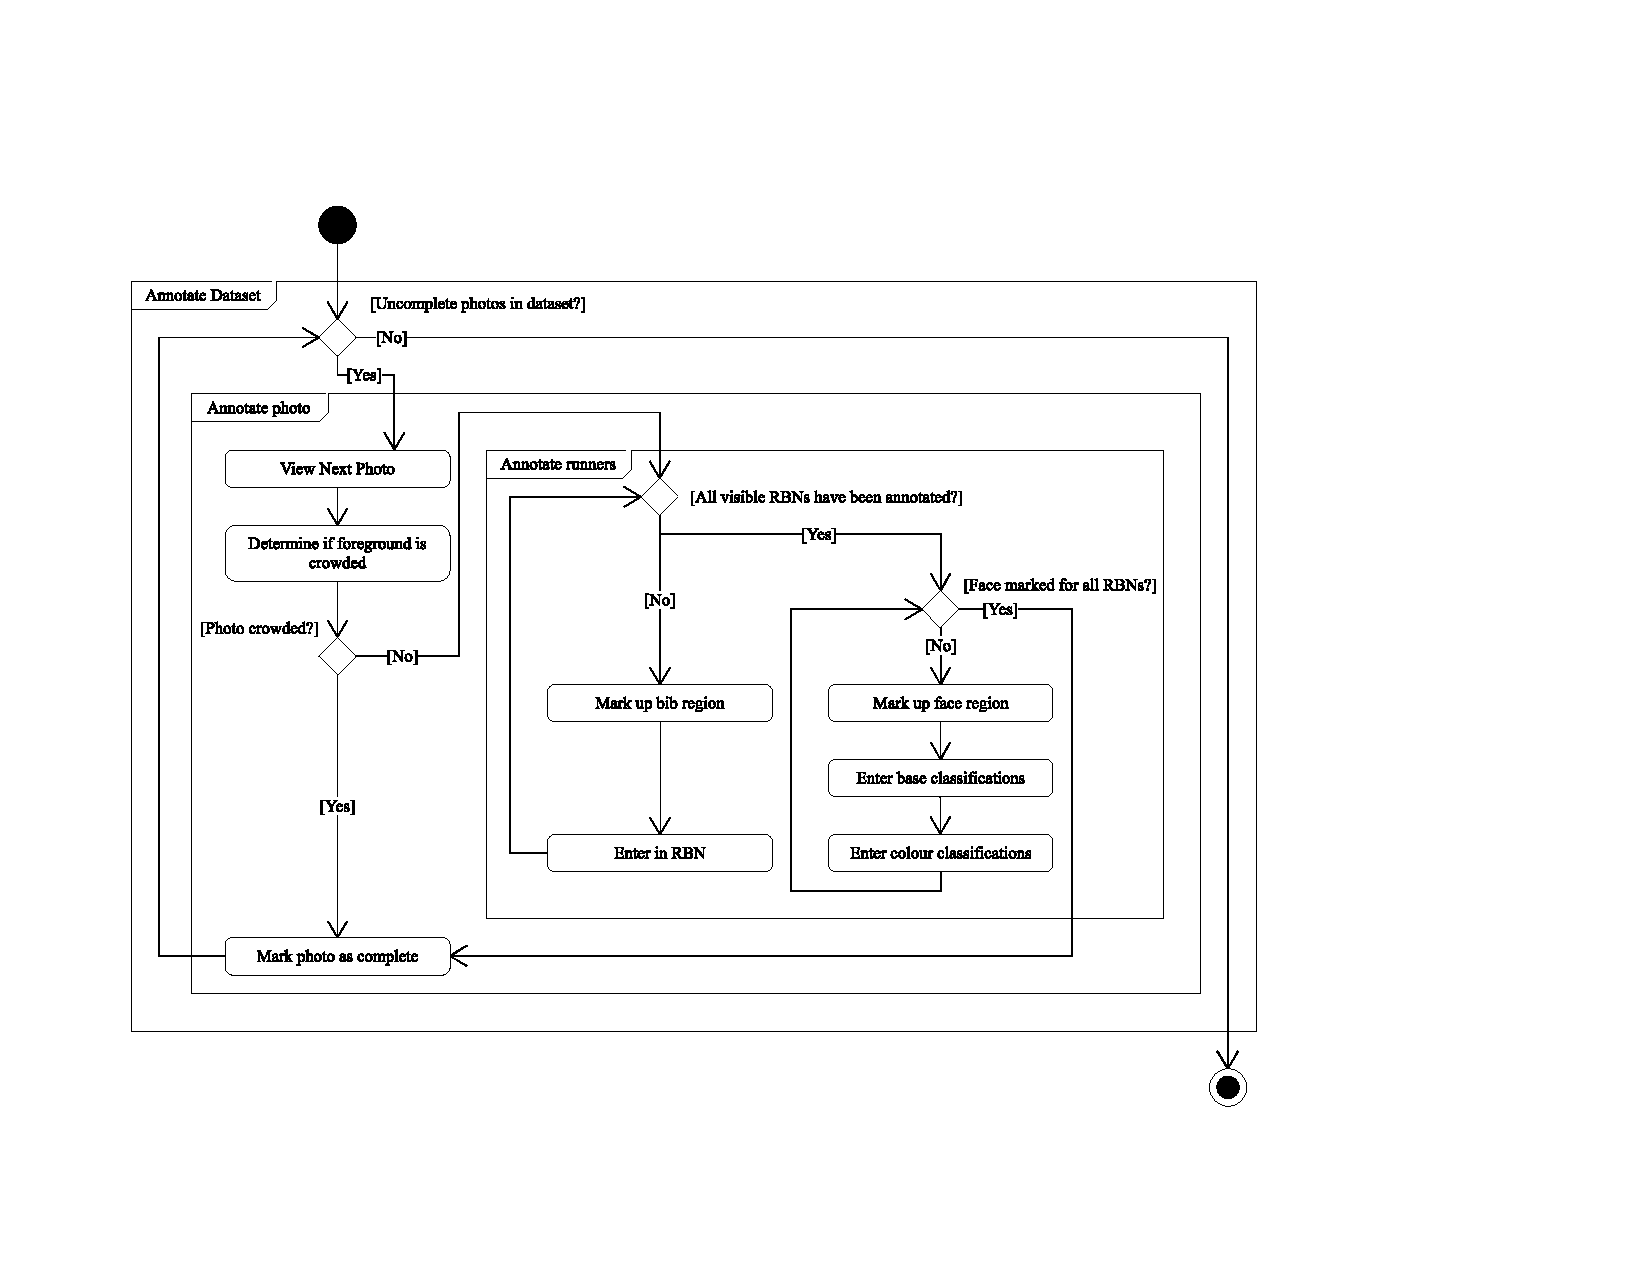
\includegraphics[width=0.9\paperwidth]{images/dataset/concrete_workflow}
  \caption[Concrete workflow example using Argus]{Concrete workflow of Argus in our bib annotation context. The \gls{acl} structures this process by defining dependency ordering.}
  \label{fig:dataset:process:argus_workflow}
\end{figure}
\end{landscape}

\subsection{Transformation}
\label{sec:dataset:process:transformation}

The features, once extracted, are encoded into an \glsx{adf} upon marking the image as complete. To prevent data loss, files are encoded as the annotator progresses onto the next feature within the workflow of extraction. All derived attributes can be calculated given the explicit attributes manually entered by the runner at this stage.

A sample of an \gls{adf} in a language-agnostic tree format is shown in \cref{fig:dataset:adf_representation} for a photo with one runner. This could be serialised into any human-readable hierarchical format (such as a \glsac{yaml}, \glsac{json}, \gls{xml} file or machine-readable compressed formats). Additionally, workflows from the \gls{acl} input file may be generated into a \gls{uml} state diagram (as we have done in \cref{fig:dataset:process:argus_workflow}) to assist annotators in understanding how to mark up the photo. Thus, the transformation step \textit{universalises} the annotated data into a format readable by any supported parser of the \gls{adf} or \gls{acl} files. We propose examples of how this data is loaded in the following section.

\renewcommand*\DTstyle{\small\rmfamily}
\setlength{\DTbaselineskip}{15pt}

\begin{figure}
  \begin{subfigure}[b]{0.45\textwidth}
    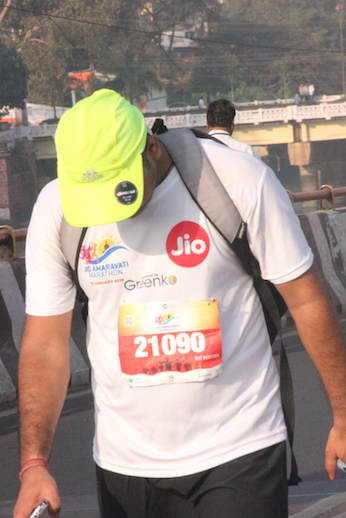
\includegraphics[width=\textwidth]{images/dataset/sample_annotated_runner}
  \end{subfigure}
  \vspace*{\fill}
  \hspace{-0.025\textwidth}
  \begin{subfigure}[b]{0.50\textwidth}
    \dirtree{%
      .1 \textbf{Image} \texttt{001}.  
      .2 PhotoCrowded : \textit{Boolean}.
      .3 \textsc{false}.
      .2 Runners : \textit{Collection}.
      .3 Runner \texttt{1}.
      .4 \textbf{Bib}.
      .5 Bounds : \textit{Polygon}.
      .6 $x_{1} = 1164, y_{1} = 2990$.
      .6 $x_{2} = 2147, y_{2} = 2990$.
      .6 $x_{3} = 2229, y_{3} = 3745$.
      .6 $x_{4} = 1215, y_{4} = 3807$.
      .5 RBN : \textit{Label}. 
      .6 \texttt{21090}.
      .4 \textbf{Face}.
      .5 Bounds : \textit{Rectangle}.    
      .6 $x_{1} = 512, y_{1} = 1034$.
      .6 $x_{2} = 1671, y_{2} = 2162$.
      .5 Gender : \textit{Category}.
      .6 \textsc{male}.
      .5 WearingHat : \textit{Boolean}.
      .6 \textsc{true}.
      .5 WearingGlasses : \textit{Boolean}.
      .6 \textsc{false}.
      .4 \textbf{Prominence}.
      .5 \gls{lop} : \textit{Category}.
      .6 \textsc{no}.
      .5 FaceVisible : \textit{Boolean}.
      .6 \textsc{false}.
      .5 Blurry : \textit{Boolean}.
      .6 \textsc{false}.
      .4 \textbf{Colours}.
      .5 ShirtColor : \textit{Color}.
      .6 $r = 255, g = 248, b = 239$.
      .5 ShoeColor : \textit{Color}.
      .6 $N/A$.
      .5 ShortsColor : \textit{Color}.
      .6 $r = 66, g = 63, b = 58$.
      .5 HatColor : \textit{Color}.
      .6 $r = 248, g = 255, b = 134$.
    }  
  \end{subfigure}
  \caption[Sample representation of an ADF]{Sample hierarchical data representation of an \gls{adf}, encoding the features (bolded) of the runner on the left. Derived attributes are removed.}
  \label{fig:dataset:adf_representation}
\end{figure}

\subsection{Load}
\label{sec:dataset:process:load}

Once the data is transformed into a consistent format (i.e., an \gls{adf}), we are able to supply it to a number of different tools. In our research, we process the \gls{adf} in four tools:

\begin{enumerate}
  \item Argus is executed in `Review' mode, whereby a second annotator reviews the parsed annotations by loading a directory containing multiple \glspl{adf}. There, they can run through a number checks to ensure the annotated data is accurate for training the \gls{ai} models.
  \item Custom augmenters load the \glspl{adf} as well as the source images to produce a number of variations on the image, essentially turning one image and its respective \gls{adf} into many variant images and \glspl{adf}. This is imperative when training our \glsx{nn}, as explained in \cref{sec:dataset:postprocessing:augmentation}.
  \item An adapter created for our \gls{nn} is used to load in an \gls{adf} and convert it into a \glsac{csv} of file paths to images, bounding boxes and labels. The \gls{nn} reads this file and uses it to learn where bib locations are in an image. This is later discussed in \cref{ch:processing_pipeline}.
  \item We used Git\footnoteurl{https://git-scm.com}{11 Aug 2017} to track changes within our \gls{adf}. The benefit of serialising the data into a text file is that any version control management software can handle provenance for us (as suggested in \cref{sec:dataset:architecture}), thereby sourcing changes in our \gls{ai} models easier by sourcing how the training data (i.e., \gls{adf} files) has derived over time.
\end{enumerate}

% GIT!



% Extract = Extract relevant features from the image
% Transform = Transform into ADF
% Load = Load by a human reviewer or into an AI or into a augmenter

% Talk about automatic mappings. e.g. drag and drop, \gls{ui} generation with descriptive labels etc. Things we can make the \gls{ui} automate
% Then discuss provenance and how we can track using git

\section{Data Postprocessing}
\label{sec:dataset:postprocessing}

Once our dataset is annotated, a number of actions can be applied---our images and annotations undergo a series of post-processing and eventually are used by the \gls{ai} model to make predictions on new datasets. We can broadly categorise these into two sections: flagging the annotations/predictions and augmenting the data. The overall process is illustrated within \cref{fig:dataset:postprocessing:overal_data_processing}.

\subsection{Flagging}
\label{sec:dataset:postprocessing:flagging}

Flagging helps indicate `check'-states that the annotated or predicted \gls{adf} data has undergone. These checks can be considered as another way in which we maintain data provenance. We have considered four states of data: (1) ground truth annotations; (2) \textit{reviewed} ground truth annotations; (3) predicted regions from an AI model; (4) \textit{validated} predictions. These help track data provenance of training and inference samples, as presented in \cref{fig:dataset:postprocessing:state_diagram_flagging} as two \gls{uml} state diagrams.

\begin{figure}[h]
  \centering
  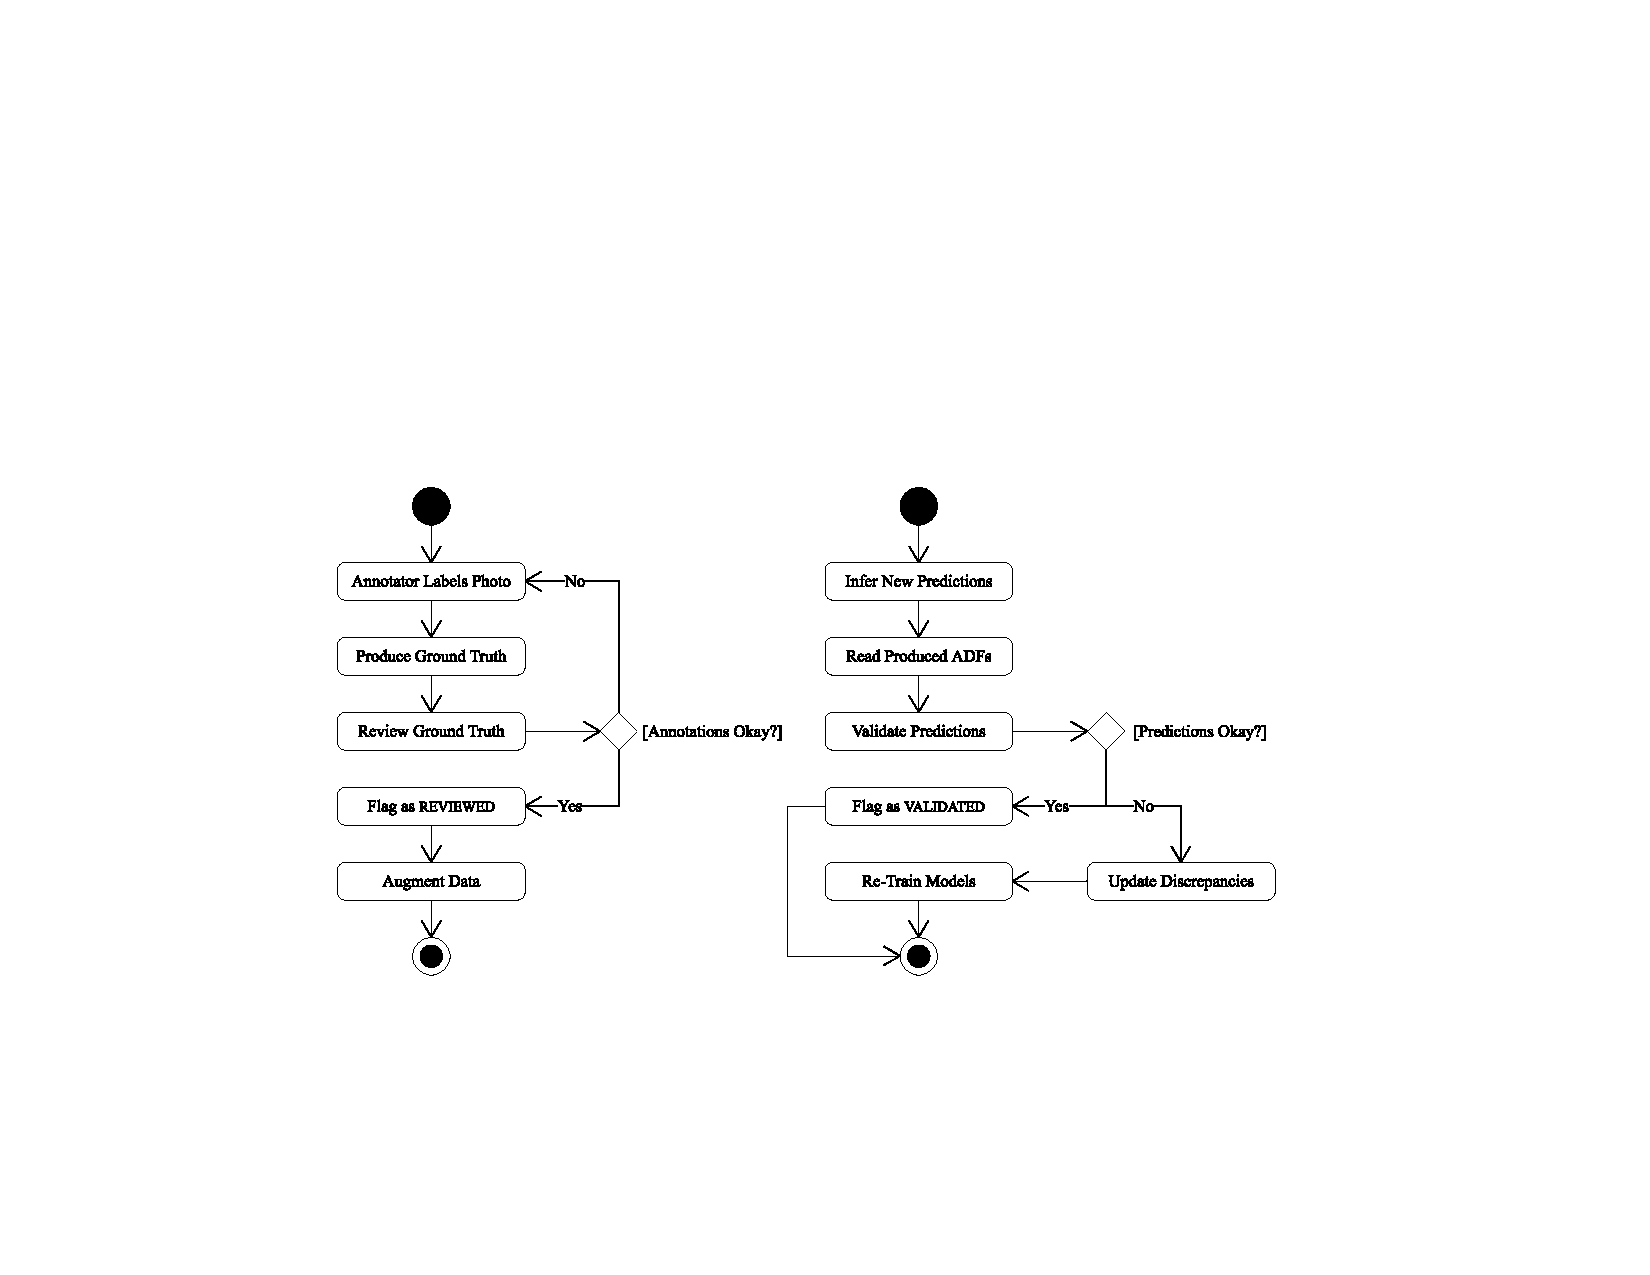
\includegraphics[width=\textwidth]{images/dataset/flagging_statemodel}
  \caption[State diagram to represent flagging]{State diagram of for training data (left) and inference data (right).}
  \label{fig:dataset:postprocessing:state_diagram_flagging}
\end{figure}

Ground truth annotations encompasses the general process by which data taggers annotate data. This process is largely the initial data capture that occurs within our dataset, described by the process outlined in \cref{sec:dataset:process}. As mentioned in \cref{sec:dataset:process:load}, once data is annotated, a second parse is done on the annotations by another reviewer to check for any mistakes. Some of our data is also annotated multiple times, and thus multiple \glspl{adf} are produced. A reviewer will check these files and use the best matches to merge the best data together---for instance, in a single photo, if three annotators mark a given runner's \gls{lop} as \textsc{yes} whereas one annotator marks it as \textsc{maybe}, the reviewer may choose to update the \textsc{maybe} to the more likely value.

Once ground truth annotations are inspected for a second time, the annotations in the \gls{adf} file are \textit{flagged} as `\textsc{reviewed}'. We only allow reviewed data to be augmented (\cref{sec:dataset:postprocessing:augmentation}) and thus trained in our \gls{ai} model. This method allows us to maintain a high level of quality and integrity of input data.

The second flag is set on \textit{predicted} \gls{adf} data generated by the \gls{ai}. As the \gls{ai} model produces \gls{adf} files (see \cref{ch:processing_pipeline}), we are able to perform a second parse on the predicted data by loading the predicted \glspl{adf} into Argus' validation mode. Here, a human validates that the predictions made by the model are indeed correct, and if not, we are able to update any discrepancies where needed (via Argus modifications) and feed this corrected invalid data into the model again to inform it of any mistakes it is making. Here we can flag the predicted data as `\textsc{validated}'. In turn, predications that are validated help ensure that mistakes made by the \gls{ai} model are amended. 

Additional flags that may be considered for future work include `\textsc{creator}', a first class concept that captures the source of who initially created the data, reviewed the data and validated the data. In doing so, quality analysis of annotators can be tracked. Furthermore, a `\textsc{merge}' flag could be considered, whereby the merge of multiple \glspl{adf} on the same source image are made. This would help track when such merges occur and how frequently they occur.

\begin{landscape}
\begin{figure}[p]
  \centering
  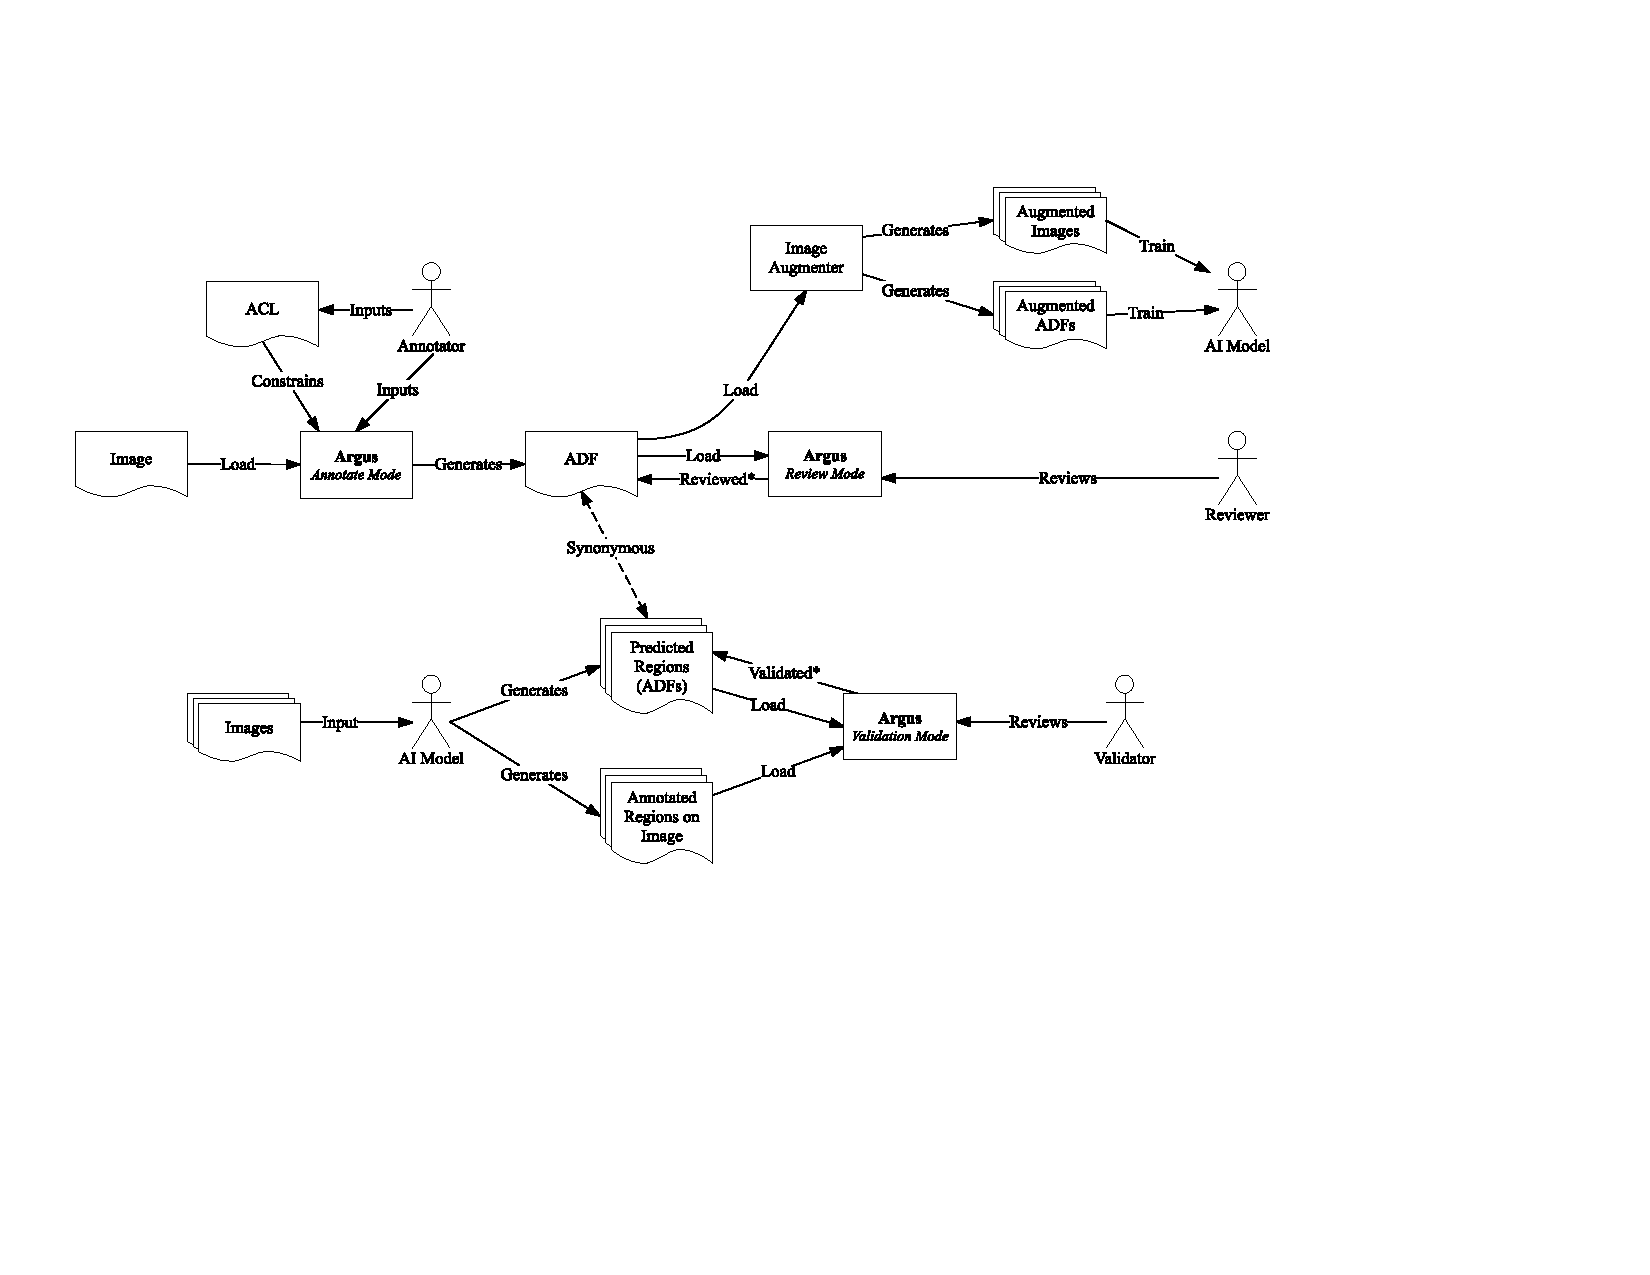
\includegraphics[width=1.1\paperwidth]{images/dataset/overview}
  \caption[Overview of processing made on our dataset]{A general outline of the processing done on the dataset and all relevant actors and associated files. Asterisks indicate where flags have marked annotations as \textsc{reviewed} and predictions as \textsc{validated}.}
  \label{fig:dataset:postprocessing:overal_data_processing}
\end{figure}
\end{landscape}

\subsection{Data Augmentation}
\label{sec:dataset:postprocessing:augmentation}

Previous works show that augmenting data makes a classifier more robust in its detection \citep{Yaeger:1996tq,Baird:1992ih,Wong:2016cv}. A solid augmentation strategy is applied to make the training data for our models more extensive and variable by generating deformations and defects and thereby producing synthetic data. We therefore motivate the need to augment our datasets by producing varied images of the same source image, rapidly fortifying our training data with more images in our dataset.

For our network, we manually tagged 803 images over a total of 14 different marathon events using our concrete Argus implementation (\cref{ch:dataset}) within our dataset. We decided on an augmentation strategy using a 1:50 ratio (thereby to produce a further 40,150 augmented images from these original 803 images). We split the dataset into 90\% for training and 10\% for validation. The specific quantities of images and annotations chosen for training and validation are described in \cref{tab:dataset:postprocessing:augmentation_quantities}. An annotation to image ratio less than 1 indicates there were more crowded photos in the sample set.

\begin{table}[t]
\centering
\caption[Breakdown of training and validation data]{Breakdown of images and annotations (runners) used for training and validation.}
\label{tab:dataset:postprocessing:augmentation_quantities}
  \tablefit{
    \begin{tabular}{@{}l|lll|lll@{}}
    \toprule
    \multirow{2}{*}{\textbf{Image Type}} & \multicolumn{3}{l}{\textbf{Training}}                                 & \multicolumn{3}{l}{\textbf{Validation}}                               \\ \cmidrule(l){2-7} 
                                         & \textbf{Images} & \textbf{Annotations} & \textbf{Annotations / Image} & \textbf{Images} & \textbf{Annotations} & \textbf{Annotations / Image} \\ \midrule
    \textbf{Original}                    & 722             & 850                  & 1.177                        & 81              & 109                  & 1.346                        \\
    \textbf{Augmented}                   & 36100           & 33098                & 0.917                        & 4050            & 4266                 & 1.053                        \\ \midrule
    \textbf{Total}                       & 36822           & 33948                & 0.922                        & 4131            & 4375                 & 1.059                        \\ \bottomrule
    \end{tabular}
  }
\end{table}

Our augmentation strategy consisted of the following:

\begin{enumerate}
  \item perform affine transformations every image,
  \item distort colour channels by adding intensities of $\pm45\%$ applied 50\% of the time,
  \item distort colour channels by multiplying intensities between a range of $[0.5, 1.5]$ applied 50\% of the time,
  \item apply one of a gaussian, average or median blur 30\% of the time.
\end{enumerate}

Our affine transformations consisted of translations in both the $x$ and $y$ axes shifted between $\pm35\%$, rotate between $\pm45\degree$, and shear between $\pm5\%$. These transformations were implemented using the \textit{imgaug} library for Python\footnoteurl{https://github.com/aleju/imgaug}{11 August 2017}. See \cref{fig:dataset:postprocessing:augmentation} for examples.

As these transformations occur randomly, there are extreme cases where translation, shearing and rotation occur extremely (e.g., \cref{fig:dataset:postprocessing:augmentation:crop1,fig:dataset:postprocessing:augmentation:crop2}). This causes some bibs to be cropped off the image. Therefore, we remove these from the transformed \gls{adf} file as we cannot have a bounding box referencing outside the image.

\begin{figure}[h!]
  \centering
  \hspace{\fill}
  \begin{subfigure}[b]{0.475\textwidth}
    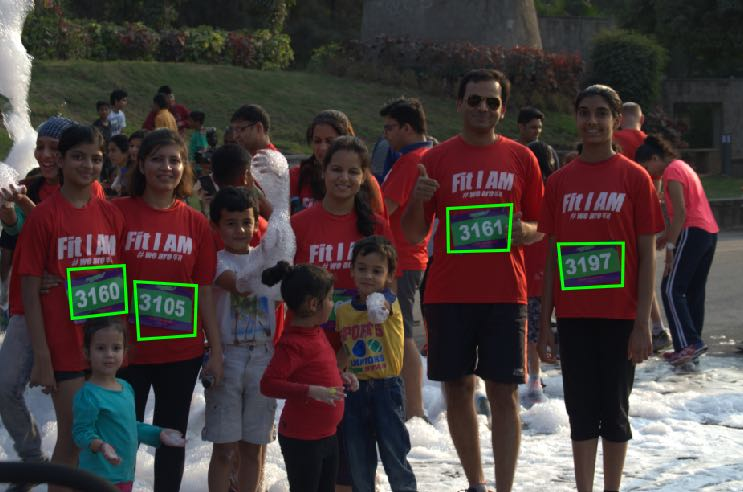
\includegraphics[width=\textwidth]{images/dataset/augmentation/original}
    \caption{Original annotated image.}
  \end{subfigure}
  \hspace{\fill}
  \begin{subfigure}[b]{0.475\textwidth}
    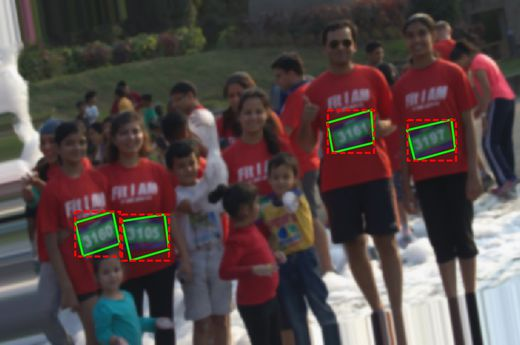
\includegraphics[width=\textwidth]{images/dataset/augmentation/slight_rotate_blur}
    \caption{Slight rotation with blur.}
  \end{subfigure}
  \hspace{\fill}
  \bigskip
  \\
  \hspace{\fill}
  \begin{subfigure}[b]{0.475\textwidth}
    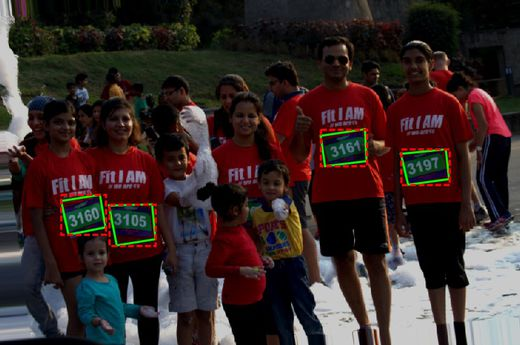
\includegraphics[width=\textwidth]{images/dataset/augmentation/neg_multiply}
    \caption{Darkened channels}
  \end{subfigure}
  \hspace{\fill}
  \begin{subfigure}[b]{0.475\textwidth}
    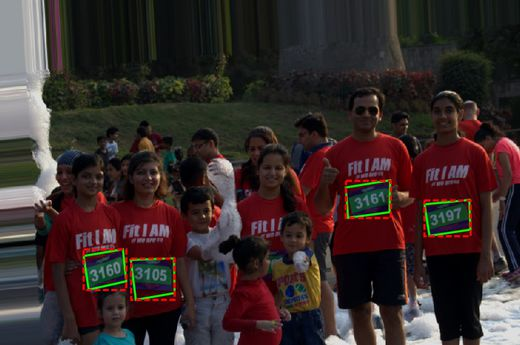
\includegraphics[width=\textwidth]{images/dataset/augmentation/offset}
    \caption{Slight translation.}
  \end{subfigure}
  \hspace{\fill} 
  \bigskip
  \\
  \hspace{\fill}
  \begin{subfigure}[b]{0.475\textwidth}
    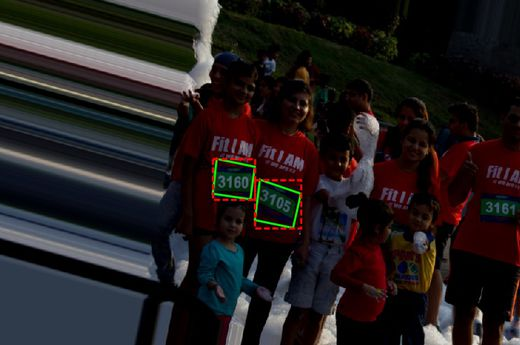
\includegraphics[width=\textwidth]{images/dataset/augmentation/dark}
    \caption{Darkened channels with translation.}
    \label{fig:dataset:postprocessing:augmentation:crop1}
  \end{subfigure}
  \hspace{\fill}
  \begin{subfigure}[b]{0.475\textwidth}
    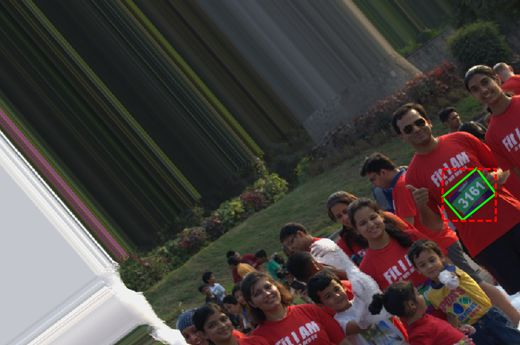
\includegraphics[width=\textwidth]{images/dataset/augmentation/large_offset_rot}
    \caption{Large translation with strong rotation.}
    \label{fig:dataset:postprocessing:augmentation:crop2}
  \end{subfigure}
  \hspace{\fill}
  \bigskip
  \\ 
  \caption[Various augmented images from our dataset]{Various instances of our augmented dataset. Here the \gls{adf} annotation files are drawn directly onto the source image, with the $BibSheet$ polygon shown in green and its respective derived bounding box attribute in red, dotted.}
  \label{fig:dataset:postprocessing:augmentation}
\end{figure}

\section{Metamodel Evaluation}
\label{sec:dataset:architecture_evaluation}

We analysed seven popular datasets recently used in literature seen as benchmarks for text extraction or object recognition. Our criteria for selection was generally open, but we ensured that usage of these datasets were from papers within at least the last 5 years. We assessed their annotation format to determine the heuristic overlap between the dataset's annotation model and our metamodel. An overview of the datasets, annotation formats and capturing software is shown in \cref{tab:dataset:metamodel_evaluation:datasets}. We summarise our analysis of directly mapping components from these formats within the \gls{adf} in \cref{tab:dataset:metamodel_evaluation:mappings}.

\vspace*{\fill}
\begin{table}[h]
  \caption[Various datasets and respective annotation formats]{Various datasets and their respective annotation formats which we have assessed for comparison with our metamodel. See \cref{ch:dataset_schemas} for serialisable annotation formats.}
  \label{tab:dataset:metamodel_evaluation:datasets}
  \tablefit{
    \begin{tabular}{@{}ll|p{0.21\textwidth}p{0.24\textwidth}lp{0.25\textwidth}@{}}
      \toprule
        \textbf{Dataset} &
        \textbf{Reference} &
        \textbf{Challenge} &
        \textbf{Format} &
        \textbf{Listing} &
        \textbf{Annotation Tooling} 
      \\
      \midrule      
        MS \glsac{coco} &
        \citep{Lin:2014vma, Chen:2015ur} &
        Object Recognition &
        MS \glsac{coco} \glsac{json} &
        \ref{lst:dataset_schemas:ms_coco} &
        Custom Tool via \glsac{amt} 
      \\
        \glsac{coco}-Text & 
        \citep{Veit:2016vj} & 
        Text Reading & 
        MS \glsac{coco} \glsac{json} & 
        \ref{lst:dataset_schemas:coco_text} & 
        Tool from \citet{Matera:2014wq} via \glsac{amt}
      \\
        \glsac{icdar} 03--11 &
        \citep{Lucas:2003iw, Lucas:2005bq, Chen:2011ul} &
        Text Reading &
        \glsac{xml} &
        \ref{lst:dataset_schemas:icdar_03-11} &
        Custom Tool via Java Applet
      \\
        \glsac{icdar} 11--15 &
        \citep{Shahab:2011hq,Karatzas:2013by,Karatzas:2015tj} &
        Text Reading &
        \glsac{xml} &
        \ref{lst:dataset_schemas:icdar_11-15} &
        \glsac{cvc} \glsac{apep} \cite{Karatzas:2014bt}
      \\
        ImageNet &
        \citep{JiaDeng:2009dl} &
        Object Recognition &
        \glsac{pascal} \glsac{voc} &
        \ref{lst:dataset_schemas:pasvoc} &
        Custom Tool via \glsac{amt}
      \\
        \glsac{sun} &
        \citep{Xiao:2010td} &
        Object Recognition &
        \glsac{pascal} \glsac{voc} &
        \ref{lst:dataset_schemas:pasvoc} &
        LabelMe \cite{Russell:2008wm}
      \\
        \glsac{pascal}-Context &
        \citep{Mottaghi:2014ie} &
        Object Recognition &
        \glsac{pascal} \glsac{voc} (2012) &
        \ref{lst:dataset_schemas:pasvoc_2012} &
        Custom Tool similar to LabelMe \cite{Russell:2008wm}
      \\
        Synth90K &
        \citep{Jaderberg:2016wj, Jaderberg:2014uy, Gupta:2016ws} &
        Text Reading &
        MATLAB Binary &
        N/A &
        SynthText\footnotemark
      \\
        \glsac{svhn} &
        \citep{Netzer:2011to} &
        Text Reading &
        MATLAB Binary &
        N/A &
        Custom Tool via \glsac{amt}
      \\
      \bottomrule
    \end{tabular}
  }
\end{table}

\footnotetext{\url{https://github.com/ankush-me/SynthText} last accessed 15 August 2017.}

\def \mmmapyes {$\bullet$}
\def \mmmapno  {\ }

\begin{table}[h]
  \caption[Components present in the ADF compared to other annotation formats]{Presence of components of popular annotation formats within the \gls{adf} metamodel. See \cref{ch:dataset_mappings} for detailed mapping.}
  \label{tab:dataset:metamodel_evaluation:mappings}
  \tablefit{
    \begin{tabular}{@{}ll|cccc@{}}
      \toprule
        \bfseries \gls{adf} &
        &
        \bfseries \glsac{coco} \glsac{json} &
        \bfseries \glsac{pascal} \glsac{voc} \gls{xml} &
        \bfseries \gls{icdar} \gls{xml} &
        \bfseries MATLAB Binaries
      \\
      \midrule
        \bfseries Feature &
        Image-Level &
        \mmmapyes{} &
        \mmmapno{} &
        \mmmapno{} &
        \mmmapno{}
      \\
        &
        Segment-Level &
        \mmmapyes{} &
        \mmmapyes{} &
        \mmmapyes{} &
        \mmmapyes{}
      \\
        \bfseries Annotation &
        Label &
        \mmmapyes{} &
        \mmmapyes{} &
        \mmmapyes{} &
        \mmmapyes{}
      \\
        &
        Category &
        \mmmapyes{} &
        \mmmapyes{} &
        \mmmapyes{} &
        \mmmapno{}
      \\
        &
        Collection &
        \mmmapno{} &
        \mmmapyes{} &
        \mmmapyes{} &
        \mmmapyes{}
      \\
        &
        Boundary &
        \mmmapyes{} &
        \mmmapyes{} &
        \mmmapyes{} &
        \mmmapyes{}
      \\
        \bfseries Attribute &
        Derived &
        \mmmapyes{} &
        \mmmapyes{} &
        \mmmapyes{} &
        \mmmapyes{}
      \\
        &
        Explicit  &
        \mmmapno{} &
        \mmmapno{} &
        \mmmapno{} &
        \mmmapyes{}
      \\
      \bottomrule
    \end{tabular}
  }
\end{table}
\vspace*{\fill}
\clearpage

For each of these datasets, the annotation capturing strategies differed and, similarly, the annotation was either encoded as a binary MATLAB\footnote{MATLAB is a registered trademark of The MathWorks, Inc.} file or serialised in plain text (either as \gls{xml} or \glsac{json}). In the case where annotations were serialised in \gls{xml}, a popular format was the \glsac{pascal}\footnote{\gls{pascal}}-\gls{voc} \citep{Everingham:2009dq} format. This format was made popular with the various \glsac{pascal} \gls{voc} Challenges \citep{Everingham:2015tv,Everingham:2010wz,Everingham:2005vr,Everingham:2009dq}, though custom annotation formats in \gls{xml} are also present (e.g., \gls{icdar}).

\subsection{MS COCO and COCO-Text JSON Format}

The Microsoft \gls{coco} \citep{Lin:2014vma} dataset and its image captions extension \citep{Chen:2015ur} require all annotations to be labelled to one of 91 specified categories. This is done using a three-step annotation pipeline consisting of: (1) labelling all categories of objects in the image, (2) spotting all instances of these characters, and (3) segmenting the instances using a polygon. For our analysis, we focus only on the Object Keypoint and Image Caption Annotation challenges.

We mapped the annotation concepts from both MS \gls{coco} (and its text-reading equivalent \gls{coco}-Text) and mapped components to the \gls{adf}. As shown in \cref{fig:dataset:metamodel_evaluation:mapping:coco}, these high-level components are largely complete when expressed in \gls{adf}, and the mapping is powerful enough to compute required components of the \gls{coco}-based annotation formats to derived calculations within \gls{adf}.

Our metamodel did not consider using \gls{rle} to encode multiple boundaries (polygons), as is used when \textit{Is Crowd} is set to 1 to indicate multiple instances in the image. However, we still capture this concept under the a form of a \textit{Boundary}. Additionally, we found that the \textit{Is Crowd} is the only mapping of all the formats that relates to an \gls{adf} \textit{Image-Level Feature}.

\subsection{PASCAL VOC XML Format}

The \gls{pascal} \gls{voc} \gls{xml} format showed the most consistency with \gls{adf}'s variant \textit{Annotation} sub-types (\cref{fig:metamodel_class_diagrams:feature}), along with the \gls{icdar} \gls{xml} format. The \gls{pascal} \gls{voc} format shows direct mappings to our components, such as \textit{Bounding Box} to an \textit{Annotation}'s equivalent, \textit{Boundary}. Additionally, a collection of \textit{Action}s (as given in the 2012 format to extend the \textit{Pose} of a person feature) can be used as a list of variant \textit{Category} annotations. Further mappings can be seen in \cref{fig:dataset:metamodel_evaluation:mapping:pascal}.

\subsection{ICDAR XML Formats}

The two \gls{icdar} datasets (including the 2011 update) can also be captured within an \gls{adf}. We present this mapping in \cref{fig:dataset:metamodel_evaluation:mapping:icdar}. Most notably, we map the \textit{Text Line}, \textit{Word}, \textit{Atom} and \textit{Text Parts} as \gls{adf} \textit{Collection}s. The \textit{Don't Care} component is a flag to notify if a line is illegible, which we can indicate using a \textit{Boolean} annotation (a \textit{Category}). The explicit \textit{Color} type in the \gls{icdar} 2011--2015 format can also be mapped to a \textit{Label} (more specifically, the \textit{Colour} label).

\subsection{MATLAB-Encoded Binaries}

To investigate the mapping of variant MATLAB binaries, we inspected the relevant guides on how to read the cell-arrays for both the SynthText 90k\footnoteurl{http://www.robots.ox.ac.uk/~vgg/data/scenetext/readme.txt}{17 August 2017} and \gls{svhn}\footnoteurl{http://ufldl.stanford.edu/housenumbers/\#downloads}{17 August 2017} datasets. Of the formats investigated, these were the simplest, and were the only ones to directly map an \textit{Explicit Attribute} (for Synth90k). These are shown in further detail within \cref{fig:dataset:metamodel_evaluation:mapping:matlab}.

% Evaluate the meta model using a herustic overlap to check if our metamodel is complete. Do this against three existing and popular datasets: COCO text, ICDAR?, SVHN?. Check Scott's thesis on his eval strats to see if the metamodel is complete, consistsent and expressive enough against other parts of the meta model, and where we could potentially fill gaps.

% COCO Text \cite{}, MS Coco  \cite{} (JSON)

% ICDAR03-11 XML (\cite{Lucas:2005hl})

% ImageNet \cite{JiaDeng:2009dl}, stored in the PASCAL-VOC Format

% Synth90k \cite{Gupta:2016ws}
% http://www.robots.ox.ac.uk/~vgg/data/scenetext/SynthText.zip
% Bounding Boxes (x y)
% SynthText.zip (size = 42074172 bytes (41GB)) contains 858,750 synthetic
%scene-image files (.jpg) split into 200 directories, with 
%7,266,866 word-instances, and 28,971,487 characters.
%
%Ground-truth annotations are contained in the file "gt.mat" (Matlab format).
%The file "gt.mat" contains the following cell-arrays, each of size 1x858750:
%
%  1. imnames :  names of the image files
%
%  2. wordBB  :  word-level bounding-boxes for each image, represented by
%                tensors of size 2x4xNWORDS_i, where:
%                   - the first dimension is 2 for x and y respectively,
%                   - the second dimension corresponds to the 4 points
%                     (clockwise, starting from top-left), and
%                   -  the third dimension of size NWORDS_i, corresponds to
%                      the number of words in the i_th image.
%
%  3. charBB  : character-level bounding-boxes,
%               each represented by a tensor of size 2x4xNCHARS_i
%               (format is same as wordBB's above)
%
%  4. txt     : text-strings contained in each image (char array).
%               
%               Words which belong to the same "instance", i.e.,
%               those rendered in the same region with the same font, color,
%               distortion etc., are grouped together; the instance
%               boundaries are demarcated by the line-feed character (ASCII: 10)
%
%               A "word" is any contiguous substring of non-whitespace
%               characters.
%
%               A "character" is defined as any non-whitespace character.

% SVHN \cite{Netzer:2011to} - Each element in digitStruct has the following fields: name which is a string containing the filename of the corresponding image. bbox which is a W array that contains the position, size and label of each digit bounding box in the image. Eg: digitStruct(300).bbox(2).height gives height of the 2nd digit bounding box in the 300th image. 

% SUN \cite{Xiao:2010td}; http://people.csail.mit.edu/torralba/publications/memories.pdf <- annotation
% Scene recognition. Does not specify their annotation language for aspects within a scene.  
% LabelMe annotation tools.

%%%% 

% Evaluate argus UI with others, such as the annotation of COCO in the COCO dataset paper (Fig 12).

% SUN - http://labelme.csail.mit.edu/Release3.0/browserTools/php/matlab_toolbox.php; http://people.csail.mit.edu/brussell/research/AIM-2005-025-new.pdf

% - https://docs.scaleapi.com/#polygon-annotation
%% Large annotation 
%% Annotation as a service


\newpage
\section{Conclusions}

This chapter describes an inductive approach used for developing a generalisable metamodel from empirical iterations of systems development to gap the missing epistemology in the area of data capturing architectures. By developing a concrete implementation and reflecting upon the implementation, we were able to refine and discover a concrete metamodel. This metamodel alleviates the difficulties in maintaining data provenance when training \gls{ai} models by making the serialisable, the therefore trackable with version control systems.

How may this metamodel be used elsewhere? It seems easily adaptable to similar areas in the field of computer vision processing, such as \gls{lpr} or \gls{tsr}. However, could we move this to beyond static images? Future works may extend our metamodel to multiple image frames, and therefore annotating videos frame-by-frame is within reach. Some current limitations of the metamodel (in its current form) is the difficulty to apply it to non-vision-related topics, such as \gls{nlp}, audio processing or sensor data processing. Some key concepts may be missing from our metamodel in these areas, and we expect that these can be closed by researchers with relevant domain expertise who can further extend it. We also propose that our approach could be used as a background for future works in metamodel development.

Additionally, we have shown that our metamodel is consistent with four popular existing data formats, and therefore is aligned to requirements of previous annotation systems. Hence, adapters can be used to map such formats, thereby unifying all datasets into one readable format which can be used for \gls{ai} training and validation. We leave this open for future work.

\bigskip

\noindent
The primary contributions of this chapter are:

\begin{itemize}
  \item an approach to define prominence of marathon runners that is quantifiable,
  \item a metamodel that describes a schema to annotate large image datasets, and
  \item an exploratory methodological approach in designing a metamodel from a concrete system.
\end{itemize}

\noindent
Minor contributions in this chapter include:

\begin{itemize}
  \item a basic comparison of our metamodel against existing image-based datasets, and
  \item an overall pipeline in how to handle and deal with data provenance in \gls{ai} models.
\end{itemize}

% Concluding remarks:
% - Speculate if this metamodel is extensible?
% -- Videos?
% -- Audio?
% -- LIDAR + RFID / Sensor Data?
% - Is the methodological approach extendable?
% -- Using a concrete system to redevelop back toward a metamodel?
% - Perhaps compare with how ICDAR was annotated
% - Compare with the online websites... like integrating with Scale and the other thing?
% - "Left for future research"


% motivation
% methodology
% a layered data tagging metamodel
%% definitions (data structures)
%% layering
%% workflows
% implementation
%% findings (productivity)
%% quality
